%%%%%%%%%%%%%%%%%%%%%%%%%%%%%%%%%%%%%%%%%%%%%%%%%%%%%%%%%%%%%%%%%
%%% %
%%% % weiiszablon.tex
%%% % The Faculty of Electrical and Computer Engineering
%%% % Rzeszow University Of Technology diploma thesis Template
%%% % Szablon pracy dyplomowej Wydziału Elektrotechniki 
%%% % i Informatyki PRz
%%% % June, 2015
%%%%%%%%%%%%%%%%%%%%%%%%%%%%%%%%%%%%%%%%%%%%%%%%%%%%%%%%%%%%%%%%%

\documentclass[12pt,twoside]{article}

\usepackage{raport}

\author{Damian Bielecki}

% np. EF-123456, EN-654321, ...
\studentID{EF-163461}
\title{Śledzenie obiektów przez robota mobilnego z wykorzystaniem głębokiej sieci neuronowej}
\titleEN{Temat pracy po angielsku}


%%% wybierz rodzaj pracy wpisując jeden z poniższych numerów: ...
% 1 = inżynierska	% BSc
% 2 = magisterska	% MSc
% 3 = doktorska		% PhD
%%% na miejsce zera w linijce poniżej
\newcommand{\rodzajPracyNo}{1}


%%% promotor
\supervisor{dr.hab.inż Krzysztof Wiktorowicz prof. PRz}
%% przykład: dr hab. inż. Józef Nowak, prof. PRz

%%% promotor ze stopniami naukowymi po angielsku
\supervisorEN{(academic degree) Imię i nazwisko opiekuna}

\abstract{Treść streszczenia po polsku}
\abstractEN{Treść streszczenia po angielsku}

\begin{document}

% strona tytułowa
\maketitle

\blankpage

% spis treści
\tableofcontents

\clearpage
\blankpage

\section{Wprowadzenie}

Obserwując rynek możemy zauważyć ciągły wzrost liczby urządzeń będących coraz bardziej inteligentnych
i odpornych na ciągle zmieniające się otoczenie.

Celem projektu inżynierskiego jest zbudowanie robota śledzącego wskazany obiekt, który jest wykryty przez zamontowaną na nim kamerę.
Robot będzie sterowany przez komputer przetwarzający obraz przy pomocy odpowiednio wytrenowanej
głębokiej sieci neuronowej. Zadaniem sieci będzie rozpoznanie i zlokalizowanie wyznaczonego obiektu, 
a następnie przekazanie jego pozycji algorytmu sterującego. Dalsza część programu
wyśle odpowiednio spreparowane komendy do robota, aby ten ustawił karetkę z kamerą na obiektem.

Głównym powodem realizacji takiego tematu jest chęć poznania działania i trenowania głębokich sieci 
neuronowych rozpoznających obiekty na obrazach.

\textbf{Omówienie rozdziałów}

Mając na uwadze zakres pracy i cel projektu, jej treść podzielono na szereg rozdziałów. 
Rozdział pierwszy ogólnie omawia typy i zasadę działania sieci neuronowych. 
Rozdział drugi skupia się na przeglądzie literatury, a w szczególności na opisie istniejących rozwiązań
wykorzystujących rozpoznawanie obiektów przy pomocy głębokiej sieci neuronowej.
Rozdział trzeci szczegółowo omawia proces budowy wykorzystywanego dalej robota.
Rozdział czwarty opisuje proces pozyskania danych i trenowania sieci rozpoznającej obiekty.
Rozdział piąty omawia utworzony program wykorzystujący wytrenowaną sieć neuronową, cały proces sterowania i 
sposób połączenia wszystkich systemów w działający projekt.
Ostatni rozdział przedstawia testy finalnej wersji programu oraz ich krótki opis. 


\section{Omówienie działania głębokich sieci neuronowych}
\subsection{Wprowadzenie do sieci neuronowych}

Podstawowymi elementami strukturalnymi, z których buduje się sztuczne sieci 
neuronowe są neurony. Każdy neuron posiada wejścia, na które podawane są 
sygnały mnożone przez odpowiednie wagi, sumowane, a następnie po przejściu przez 
funkcje aktywacji kierowane na wyjście neuronu. 


\begin{figure}[H]
	\centering
	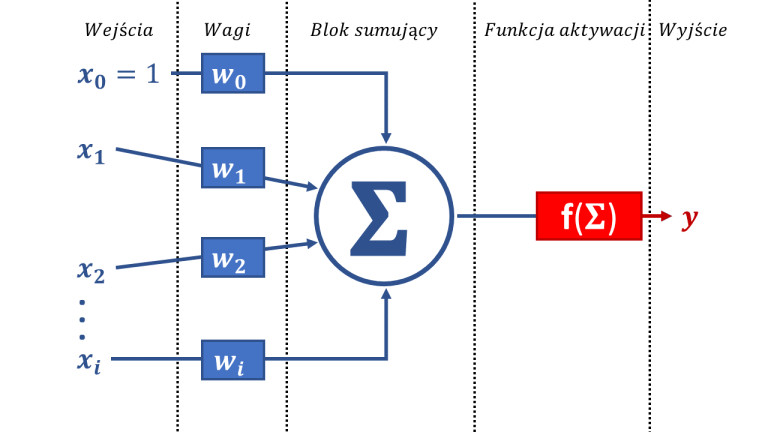
\includegraphics[width=12cm]{pages/teoria/zdjecia/sztucznyNeuron.jpg}
	\caption{Schemat pojedynczego neuronu \cite{sztucznyNeuron}}
	\label{rys:ogolnyRozwiazania}
\end{figure}


Wyjście powyższego neuronu możemy opisać wzorem:

\begin{equation}
	y = f( \sum_{i = 0}^{N}w_i x_i) = f(W^T x)
	\label{eq:rownanieNeuronu}
\end{equation}
Gdzie: $x=[1, x_1, x_2, ..., x_N]$ - to wektor sygnałów wejściowych (1 na początku wektora odpowiada
za przesunięcie), $W = [w_0, w_1, w_2, ..., w_N]$ - jest wektorem wag ($w_0$ to wartość progowa aktywacji),
$f(x)$ to wybrana funkcja aktywacji

\textbf{Najczęściej stosowane funkcje aktywacji:}

\begin{equation}
	f(x) = \frac{1}{1 + e^-x\beta} 
	\label{eq:signum}
\end{equation}

\begin{equation}
	f(x) = \frac{e^x - e^-x}{e^x + e^-x}
	\label{eq:tangensHiperboliczny}
\end{equation}

\begin{equation}
	f(x) = \begin{cases}
		1 & gdy x \> 0 \\
		0 & gdy x <  0
	\end{cases}
	\label{eq:skokuJednostkowego}
\end{equation}


\textbf{Wielowarstwowe sieci neuronowe}

W praktycznym zastosowaniu sieć zbudowana z jednej warstwy neuronów nie pozwoli nam na osiągnięcie satysfakcjonujących wyników.
Możemy określić dwa typy sieci pod względem ilości warstw: 
\begin{itemize}
	\item Uczenie maszynowe - zazwyczaj są zbudowane z trzech warstw (ukryta-ukryta-wyjściowa) 
	\item Głębokie uczenie - posiada dużo więcej warstw neuronów, w skomplikowanych sieciach nawet kilkaset
\end{itemize}

Relacje pomiędzy nimi przedstawia poniższy schemat
\begin{figure}[H]
	\centering
	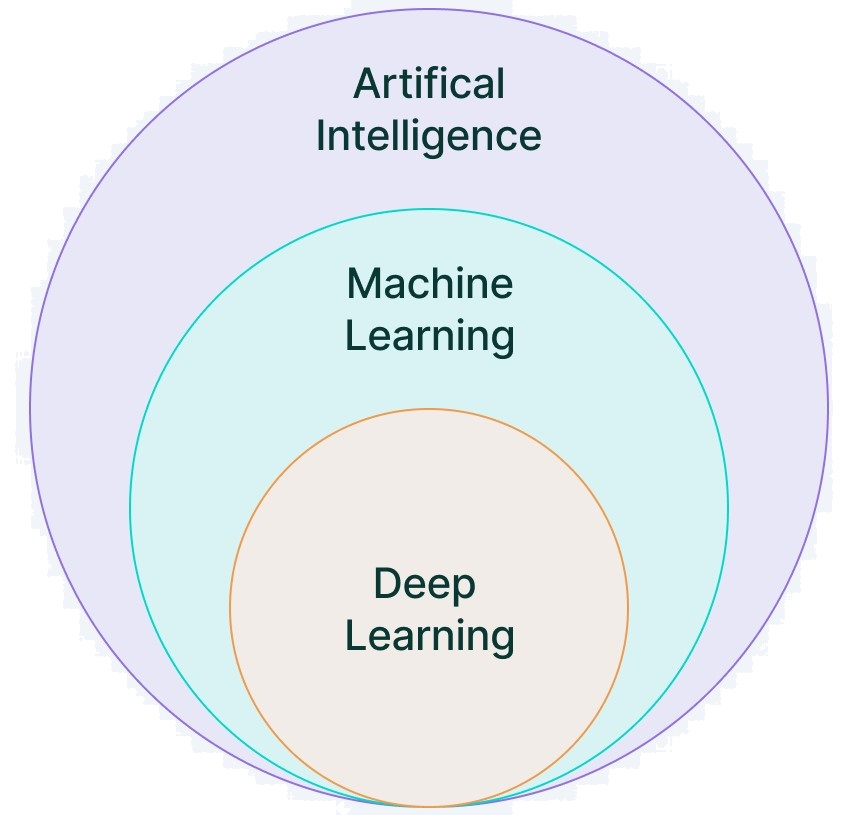
\includegraphics[width=10cm]{pages/teoria/zdjecia/schematAI.jpg}
	\caption{Relacja pomiędzy typami sieci neuronowych \cite{schematAISite}}
	\label{rys:schematAI}
\end{figure}


\subsection{Głębokie sieci neuronowe}


\subsection{Algorytmy detekcji obiektów na zdjęciach}



\section{Przegląd literatury i istniejących rozwiązań}
\subsection{Przegląd istniejących rozwiązań}
Przeglądając dostępną literature łączącą rozpoznawanie obiektów i roboty,  
można zauważyć, że takie sieci neuronowe, w dużym stopniu wspomagają analityczne algorytmy sterujące robotami. Większość artykułów opisuje mobilne roboty, których zadaniem jest poruszanie się w nieznanym środowisku. 
Pierwszy artykuł pt. "Mobile Robot Navigation Using an Object Recognition Software with RGBD Images and the YOLO Algorithm"  \cite{yoloAndMobileRobot}, opisuję wykorzystanie algorytmu YOLO do określenia przeszkód, w nieznanym otoczeniu.
Sieć neuronowa została wytrenowana na podstawie około 1100 zdjęć, zawierających: dwa typy krzeseł biurowych, stół i pudełko. Cały proces uczenia, został uruchomiony w chmurze Google i trwał około trzy dni. Aby polepszyć proces sterowania i planowania ścieżki, autorzy wykorzystali sensor Microsoft Kinect, dzięki któremu można określić rzeczywistą odległość obiektów od kamery.
Sam algorytm został uruchomiony na komputerze jedno-płytkowym Nvidia Jetson TX2 GPU, który w najgorszych warunkach przetwarzał obraz z prędkością 3,76 klatek na sekundę.

\begin{figure}[H]
	\centering
	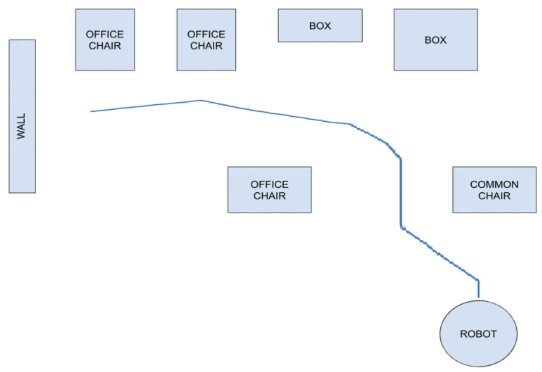
\includegraphics[width=14cm]{pages/OpisRozwiazania/img/wynikPracyArtYOLO.png}
	\caption{Ścieżka i otoczenie, w którym poruszał się robot\cite{yoloAndMobileRobot}}
	\label{rys:sciezkaRobota}
\end{figure}

Na rysunku \ref{rys:sciezkaRobota} widoczne są oznaczone przeszkody, robot oraz przebyta ścieżka. Jak widać w tym i kolejnych prezentowanych przez autorów testach, robot osiągnął docelową pozycje, mimo że nie wiedział o otaczających go przeszkodach. W zaprezentowanym rozwiązaniu, sieć neuronowa musi rozpoznać każdy otaczający robota obiekt, ponieważ w przeciwnym przypadku, ten nie uzna go za przeszkoda i go nie ominie.
W produkcyjnym rozwiązaniu przewidzenie każdego otaczającego robota obiektu jest bardzo trudne.



\subsection{Opis przyjętego rozwiązania}
Jako iż proces samego uczenia sieci neuronowej jak i jej wykorzystanie jest zbyt wymagające dla dowolnego mikrokontrolera przetwarzającego dane to algorytm wykrywający obiekty,
zostanie uruchomiony na laptopie wyposażonym w dedykowaną kartę graficzną RTX3050Ti oraz 6 rdzeniowy procesor AMD Ryzen 5 5600H. 

\begin{figure}[H]
	\centering
	\includegraphics[width=14cm]{pages/OpisRozwiazania/img/SchematOgolny.png}
	\caption{Schemat ogólny przyjętego rozwiązania}
	\label{sch:schematOgolny}
\end{figure}
Jak widać na schemacie z rysunku \ref{sch:schematOgolny}, możemy wydzielić trzy niezależne współpracujące ze sobą elementy.

\textbf{Sterownik} \newline
Zadaniem sterownika jest pobranie, odpowiednie przygotowanie obrazu (np. przeskalowanie go) i przekazanie go do algorytmu wykorzystującego głęboką sieć neuronową. 
Algorytm zwraca pozycję i etykiety wszystkich rozpoznanych na obrazie obiektów, a pozostała część programu wybiera śledzoną etykietę, wyznacza jego pozycję w przestrzeni
roboczej robota i na końcu wysyła odpowiednią komendę.


\textbf{Robot} \newline
Robot zbudowany został w oparciu o laser CNC małej mocy. Maszyna posiada dwie ruchome osie XY z karetką i przyczepionym modułem lasera. Laser i silniki krokowe sterowane są
przy pomocy sterownika opartego na płytce Arduino i odbierającym dane przy pomocy portu USB. Zamiast lasera przy pomocy wydrukowanego na drukarce 3D uchwytu została
zamocowana kamera nagrywająca przestrzeń roboczą, na której stoi urządzenie. Budowa robota została szerzej opisana w kolejnym rozdziale.


\textbf{Kamera} \newline
Jako kamera został wykorzystany telefon komórkowy z systemem Android nagrywający video w rozdzielczości 1920x1080 i 30 klatek na sekundę. W systemie została
zainstalowana aplikacja pozwalająca na strumieniowanie video przy pomocy sieci wifi co ze względu na ciągły ruch kamery znacznie uprościło jej połączenie.
W systemie Windows, na którym uruchomiona jest sieć neuronowa, telefon widoczny jest jako zwykła kamera systemowa.

\section{Budowa robota}

\textbf{Główna konstrukcja} \newline
Robot został zbudowany w oparciu o konstrukcję lasera CNC małej mocy. Główna rama, po której porusza się mocowanie z kamerą, zbudowana jest z profili aluminiowych skręconych śrubami.
Urządzenie posiada dwie sterowalne osie napędzane przy pomocy pasków maszynowych i silników krokowych. 
Konstrukcja stoi na aluminiowych nogach przymocowanych do ramy poprzez wydrukowane na drukarce 3D tuleje zaciskowe. 
Rozwiązanie to pozwala na regulację każdej nogi osobno i ustawienie poziomu. 
\begin{figure}[H]
	\centering
	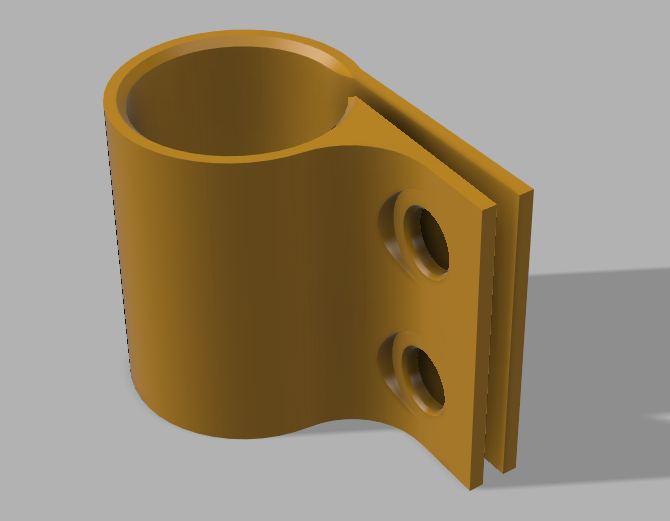
\includegraphics[height=4.5cm]{pages/dodatekARobot/img/model3DMocowaniaNog.png}
    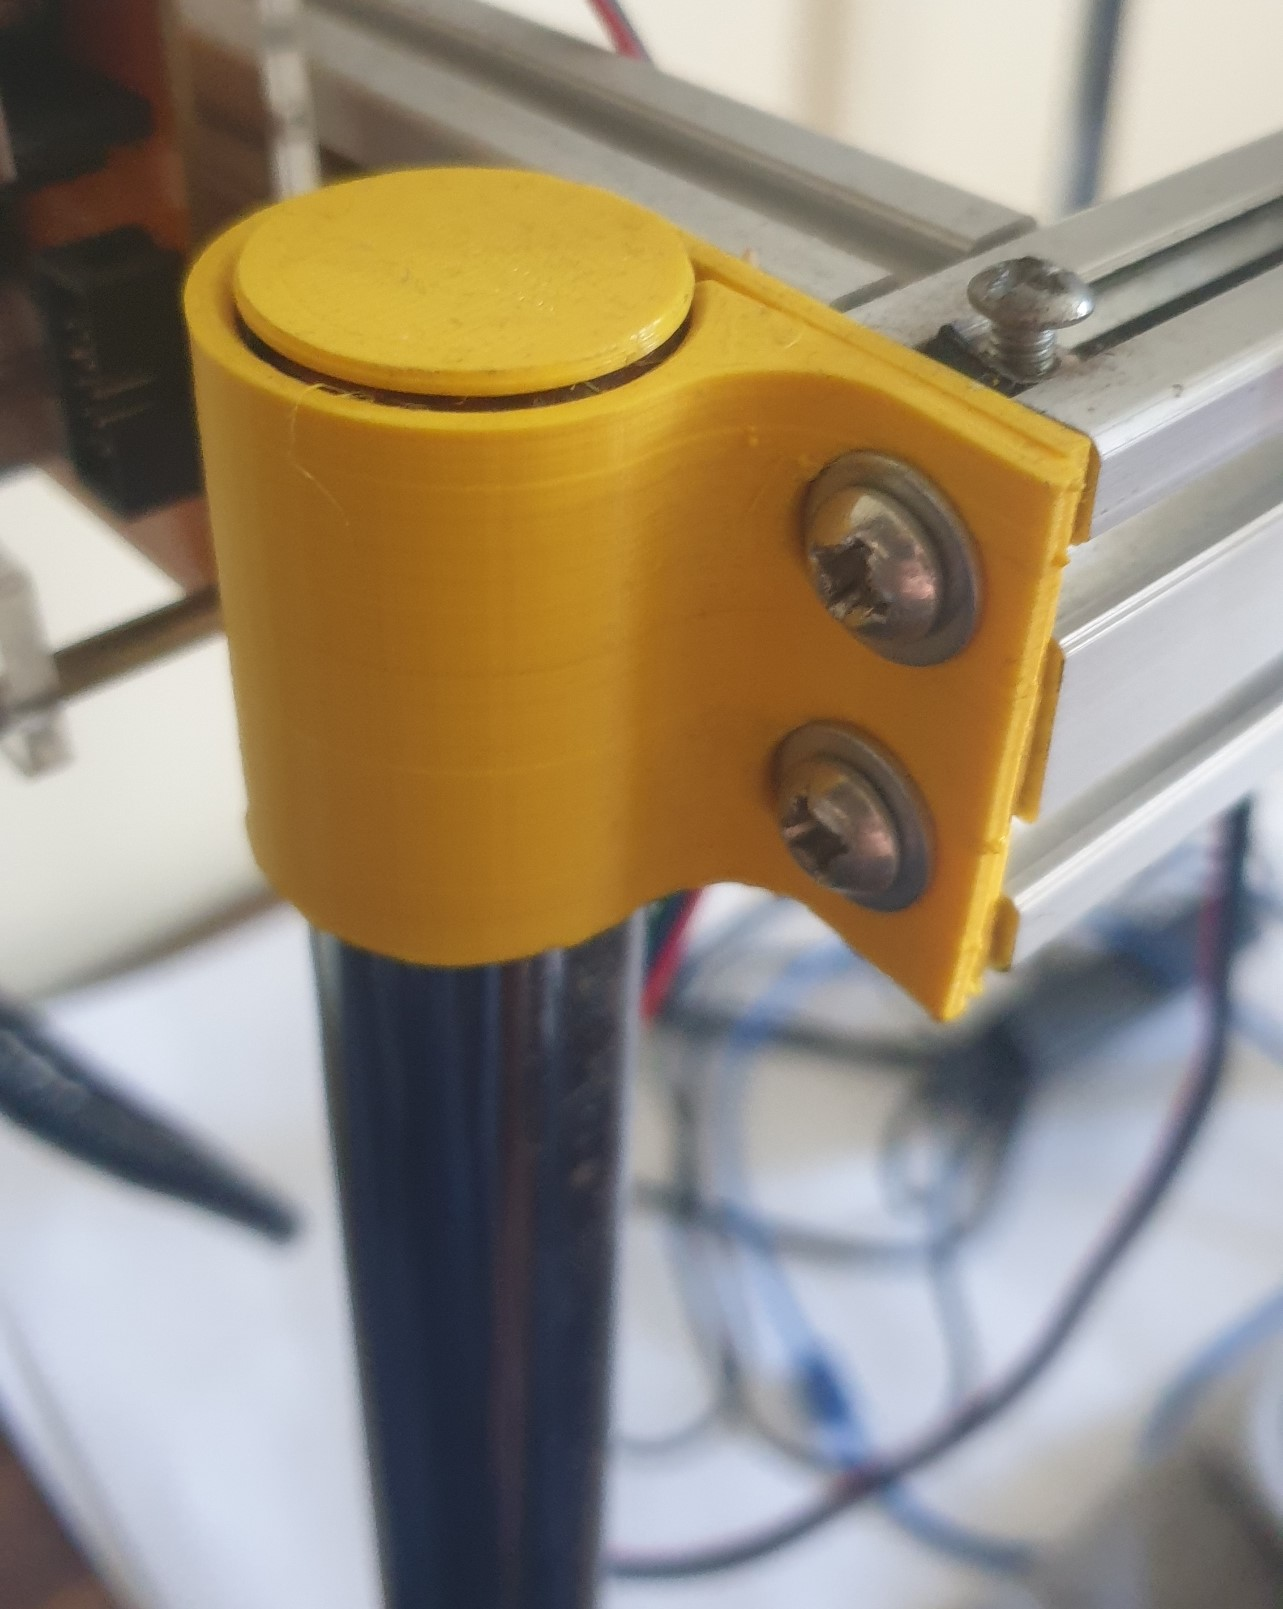
\includegraphics[height=4.5cm]{pages/dodatekARobot/img/mocowanieNogi.jpg}
	\caption{Mocowanie nóg robota, model i zdjęcie z robota}
	\label{rys:model3DMocowanieNog}
\end{figure}
Wszystkie opisywane dalej modele zostały wydrukowane z materiału 'PLA' w temperaturze ok. 210$^\circ$C i wysokością warstwy 0,15mm.

\textbf{Mocowanie kamery} \newline
Moduł z laserem został zdemontowany, a do oryginalnego uchwytu zaprojektowane zostało mocowanie telefonu, będącego w tym przypadku kamerą. 
\begin{figure}[H]
	\centering
	\begin{subfigure}{}
		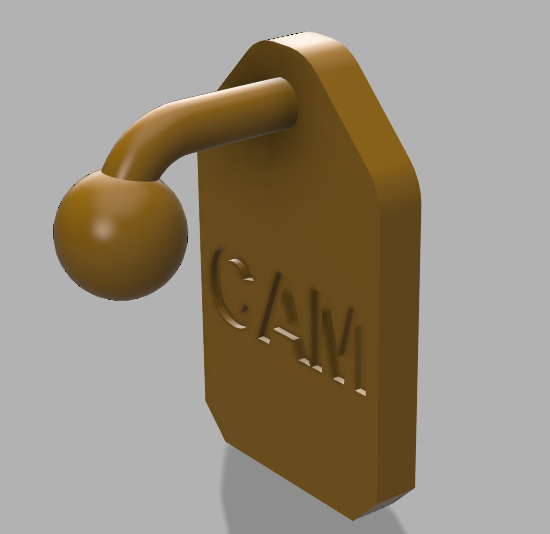
\includegraphics[height=4.5cm]{pages/dodatekARobot/img/model3DMocowaniaKamery.png}
	\end{subfigure}
	\begin{subfigure}{}
		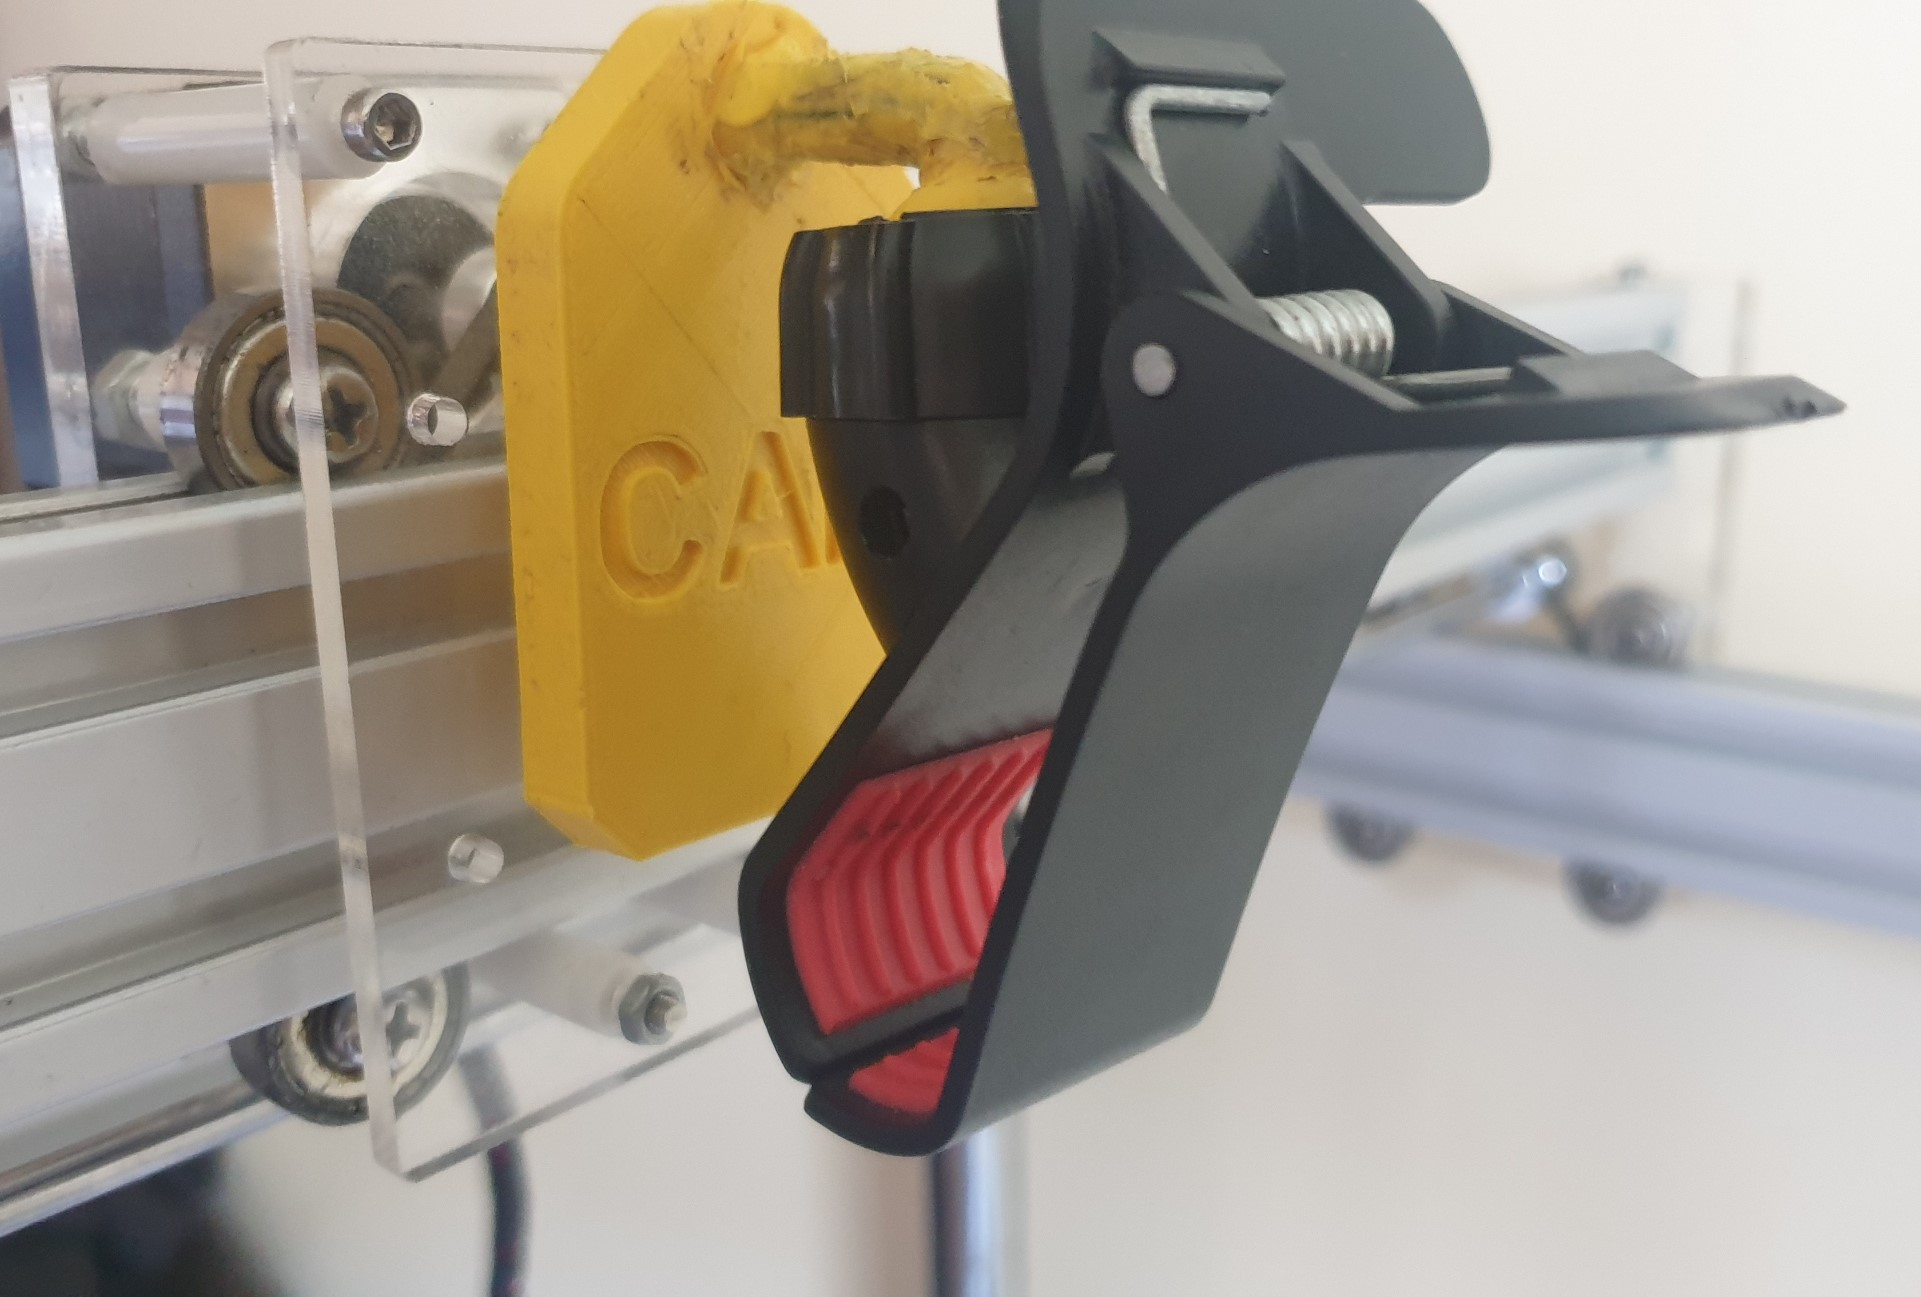
\includegraphics[height=4.5cm]{pages/dodatekARobot/img/mocowanieUchwytu.jpg}
	\end{subfigure}
	\caption{Mocowanie kamery do karetki}
\end{figure}
Do zamocowania telefonu wykorzystany został zacisk uchwytu samochodowego.
Uchwyt mocowany jest poprzez nakrętkę zaciskającą się na wydrukowanej na wysięgniku kuli. 
Takie połączenie pozwala na ustawienie kamery pod dowolnym kątem względem filmowanej powierzchni zachowując wysoką sztywność.
\begin{figure}[H]
	\centering
	\begin{subfigure}{}
		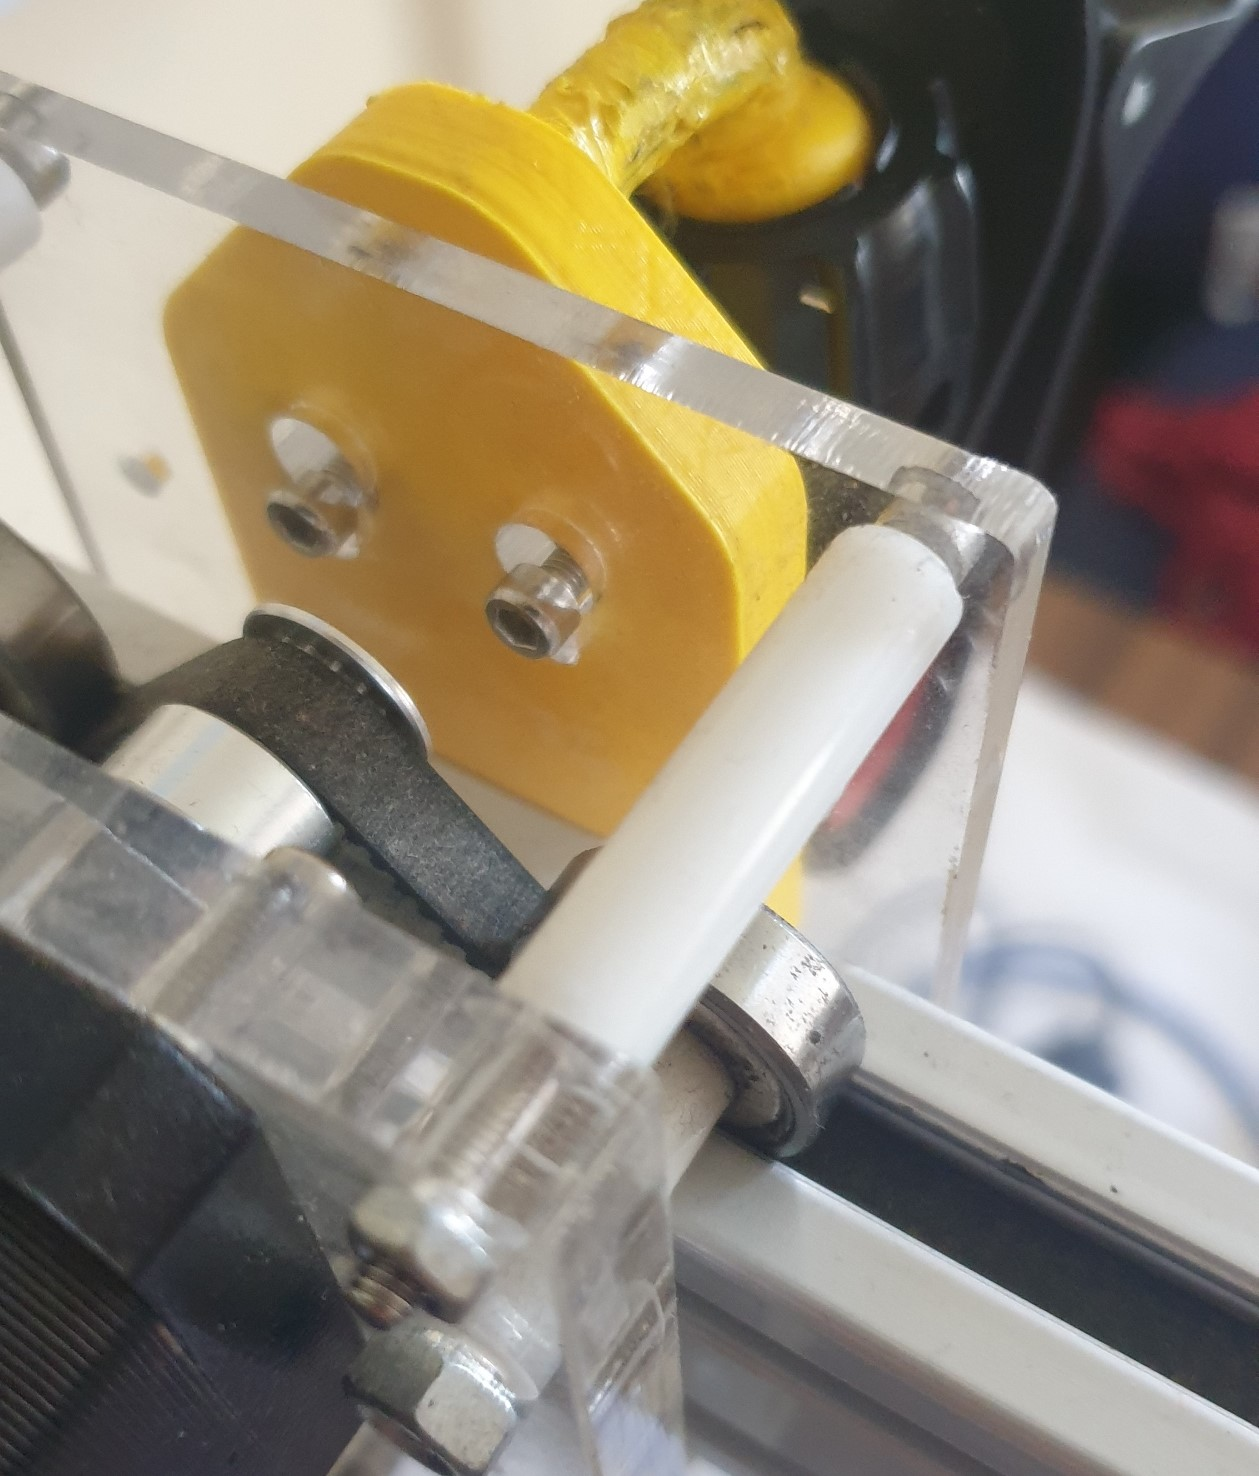
\includegraphics[height=5cm]{pages/dodatekARobot/img/mocownanieUchwytKaretka.jpg}
	\end{subfigure}
	\begin{subfigure}{}
		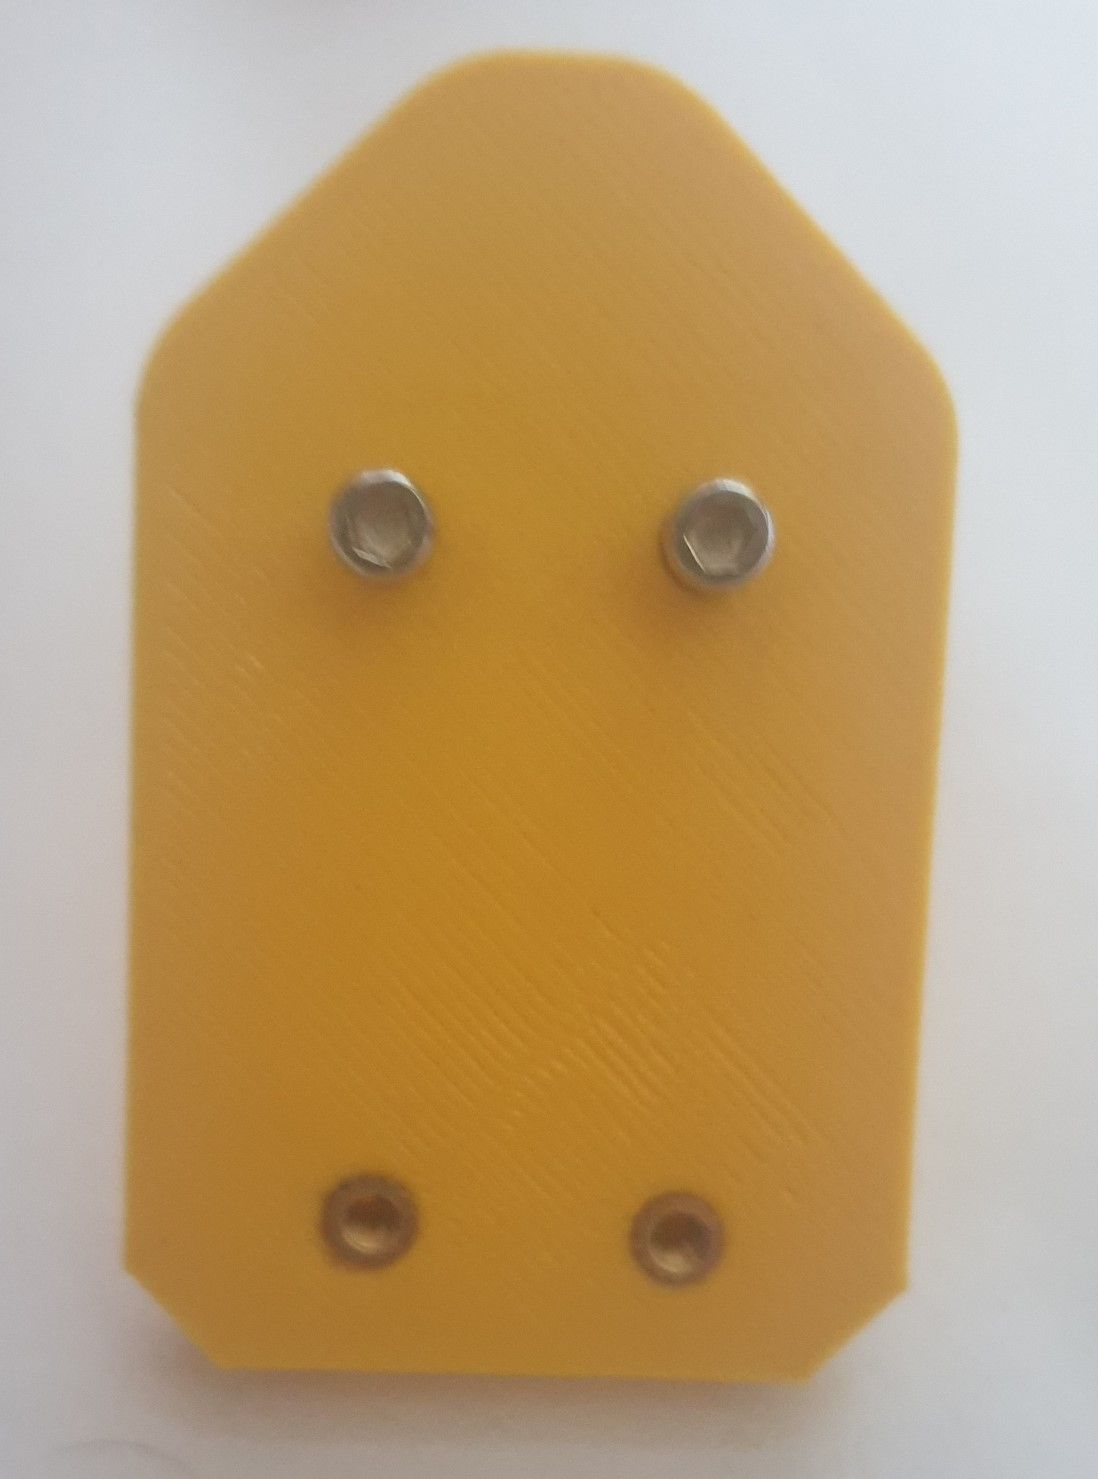
\includegraphics[height=5cm]{pages/dodatekARobot/img/mocowanieKameryTyl.jpg}
	\end{subfigure}
	\caption{Połączone mocowanie i karetka robota}
\end{figure}
Do przygotowanych otworów zostały na gorąco wciśnięte mosiężne, gwintowane tulejki, które pozwalają na wkręcenie śrub z gwintem M3.
Dzięki nim uchwyt może być sztywnie zamocowany.
Finalnie okazało się, że do sztywnego połączenia tych dwóch powierzchni wystarczą tylko dwie śruby.

\textbf{Napędy} \newline
Do napędzania obu osi robota wykorzystane zostały dwa silniki krokowe 4240-15A, o maksymalnym prądzie 1A, kroku osi 1.8$^\circ$ i maksymalnym momencie 53Ncm.
Silniki przykręcone są do grubej płyty typu 'plexa'.
\begin{figure}[H]
	\centering
	\begin{subfigure}{}
		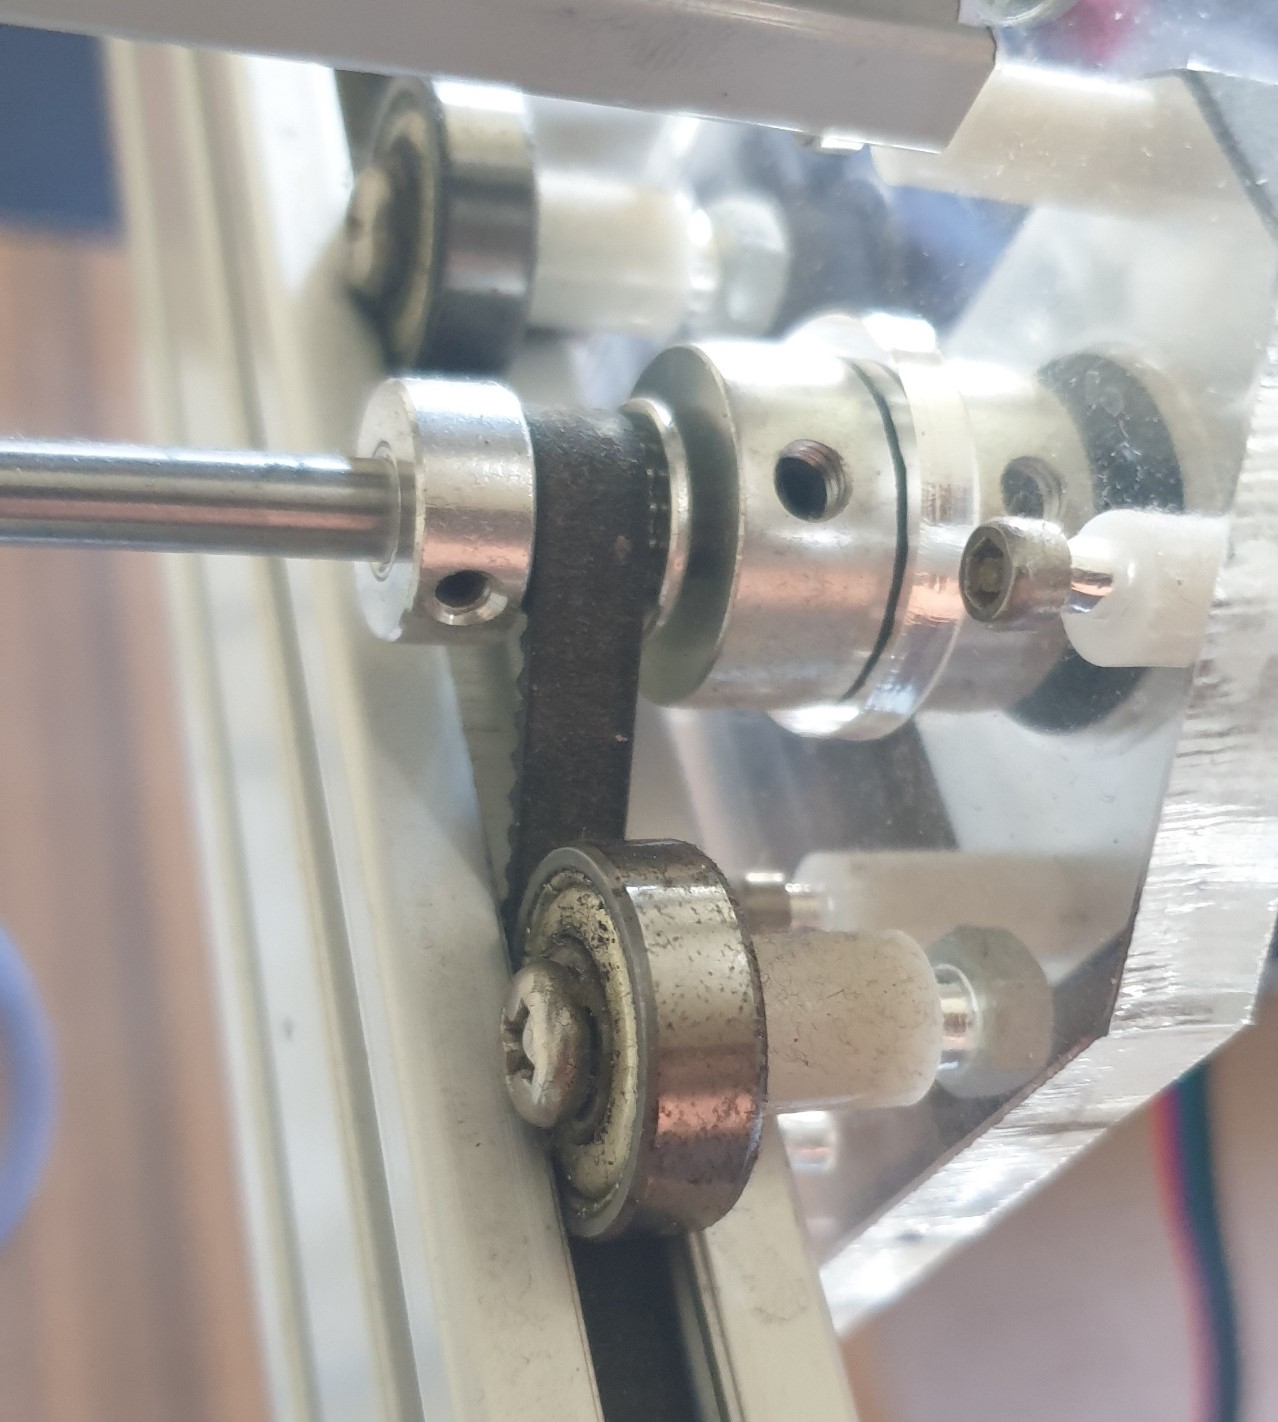
\includegraphics[height=5cm]{pages/dodatekARobot/img/przeniesienieNapedu.jpg}
	\end{subfigure}
	\begin{subfigure}{}
		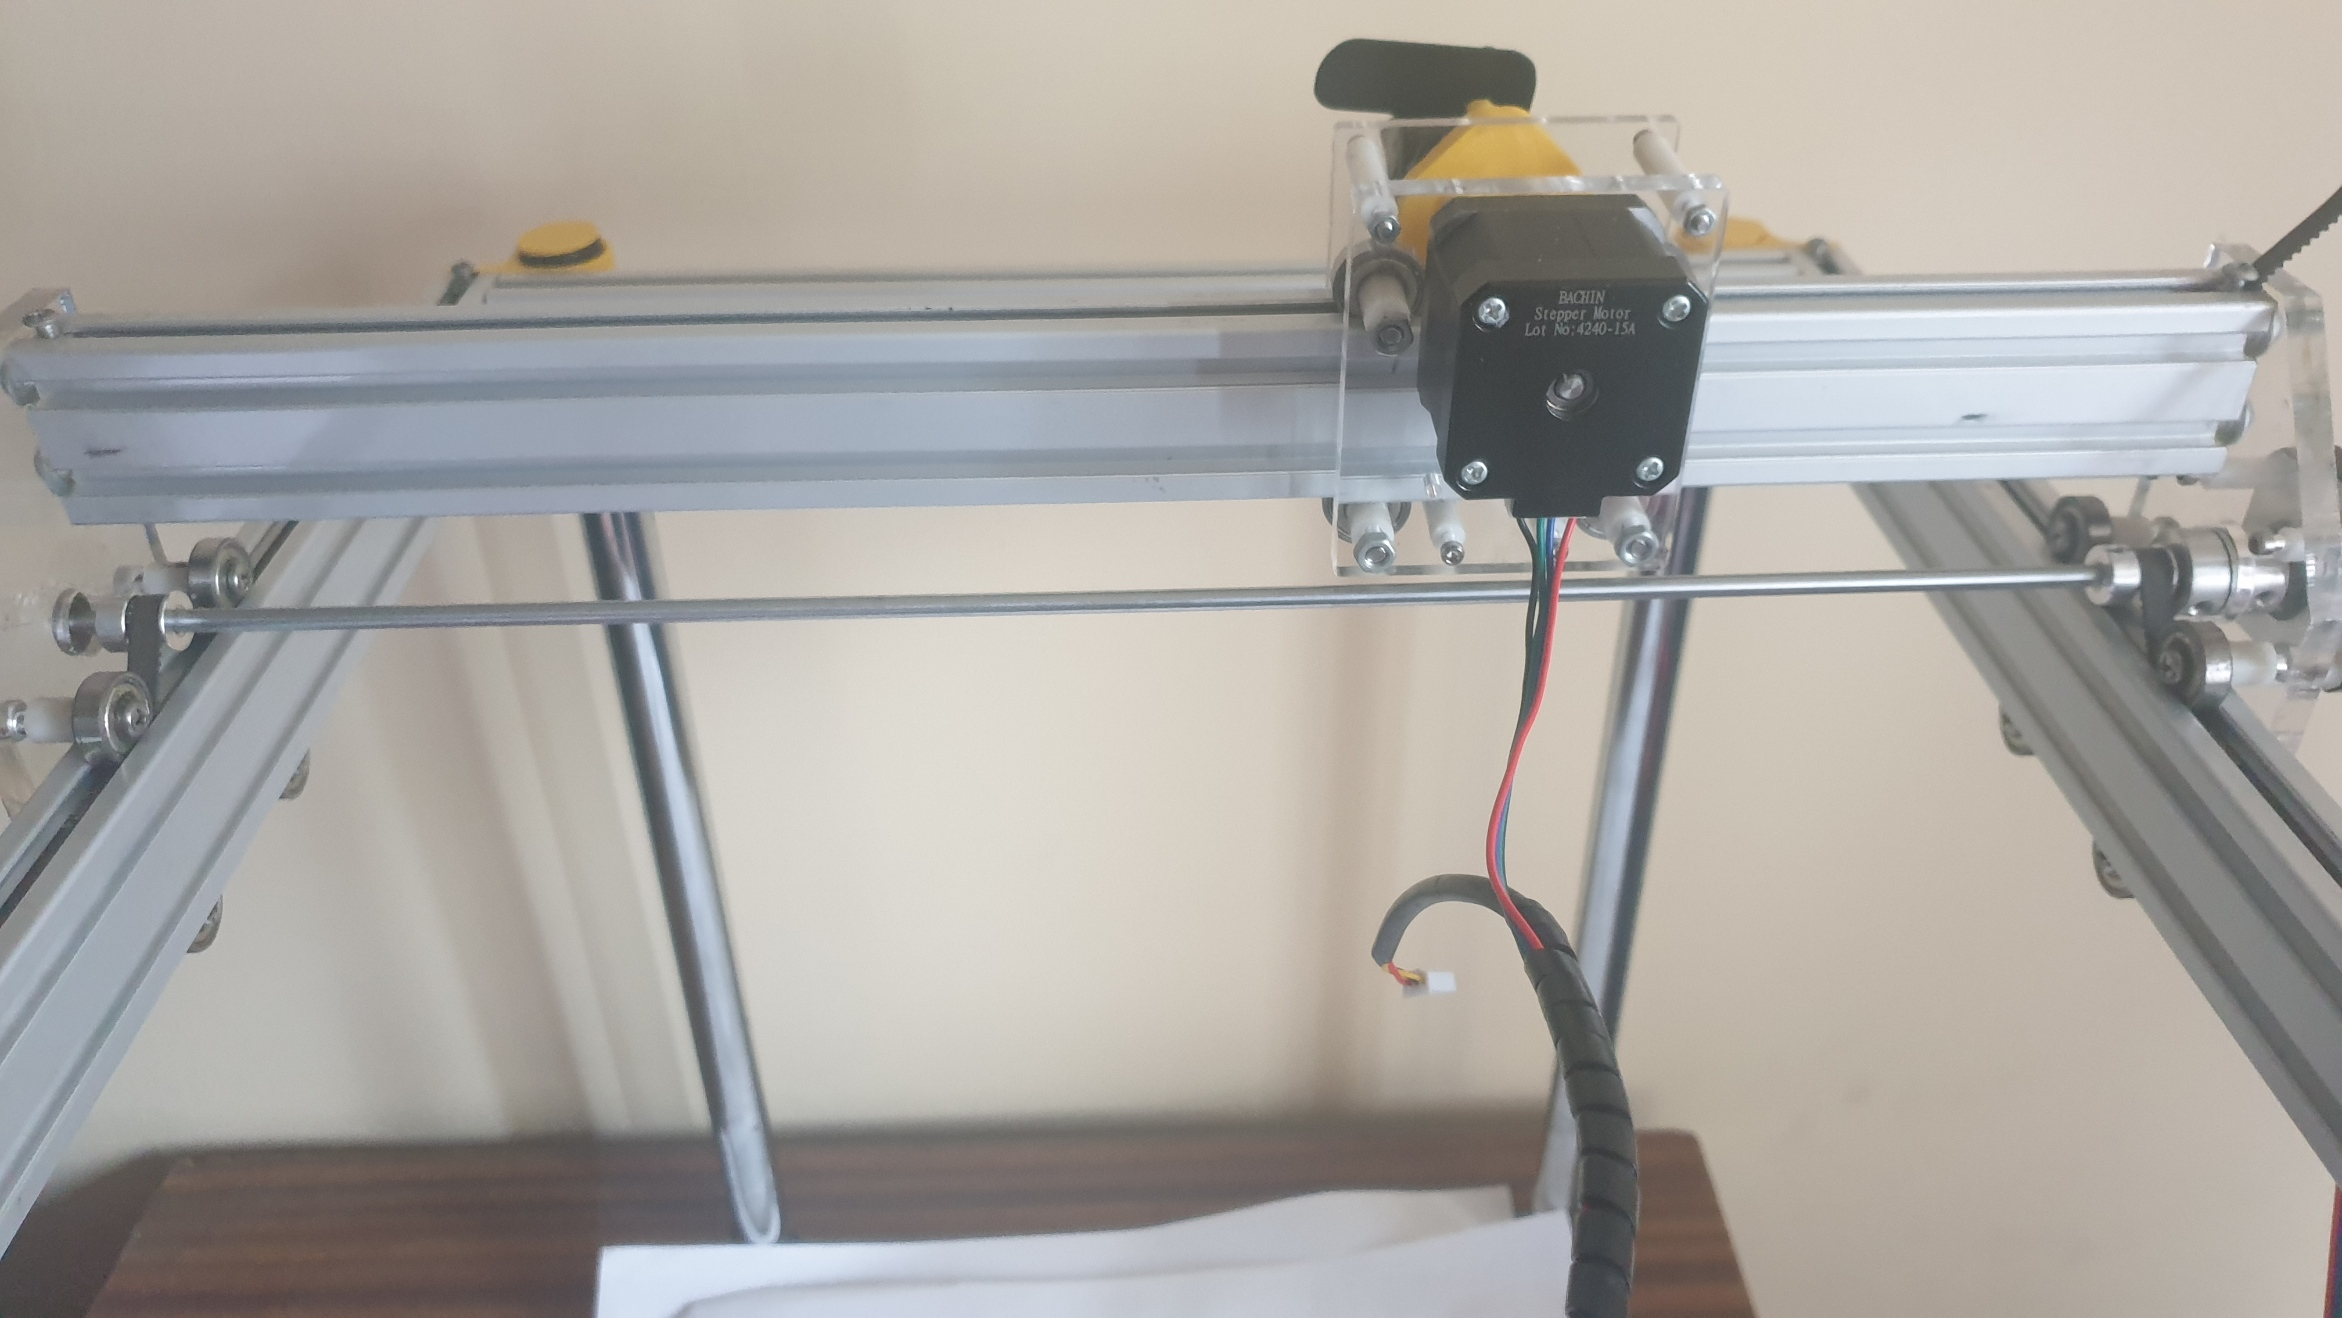
\includegraphics[height=5cm]{pages/dodatekARobot/img/ramaNapedCaly.jpg}
	\end{subfigure}
	\caption{Przekazanie napędu dla pierwszej osi}
\end{figure}
Pierwsze zdjęcie z lewej pokazuje napęd osi, po której porusza się karetka z zamocowanym kolejnym napędem. Widać że na osi silnika 
zamocowane jest sprzęgło podatne (kompensujące drgania), które połączone jest z wałkiem napędowym. 
Na obu końcach wałka zamocowane są koła zębate napędzające pasek GT-2. Pasek przymocowany jest na sztywno do ramy a naciąg kontrolowany jest przez
dwa dociskające go łożyska. Przeniesienie napędu na drugą stronę, konieczne jest ze względu na dosyć dużą ramę i możliwe skrzywianie się podczas ruchu.
\begin{figure}[H]
	\centering
	\begin{subfigure}{}
		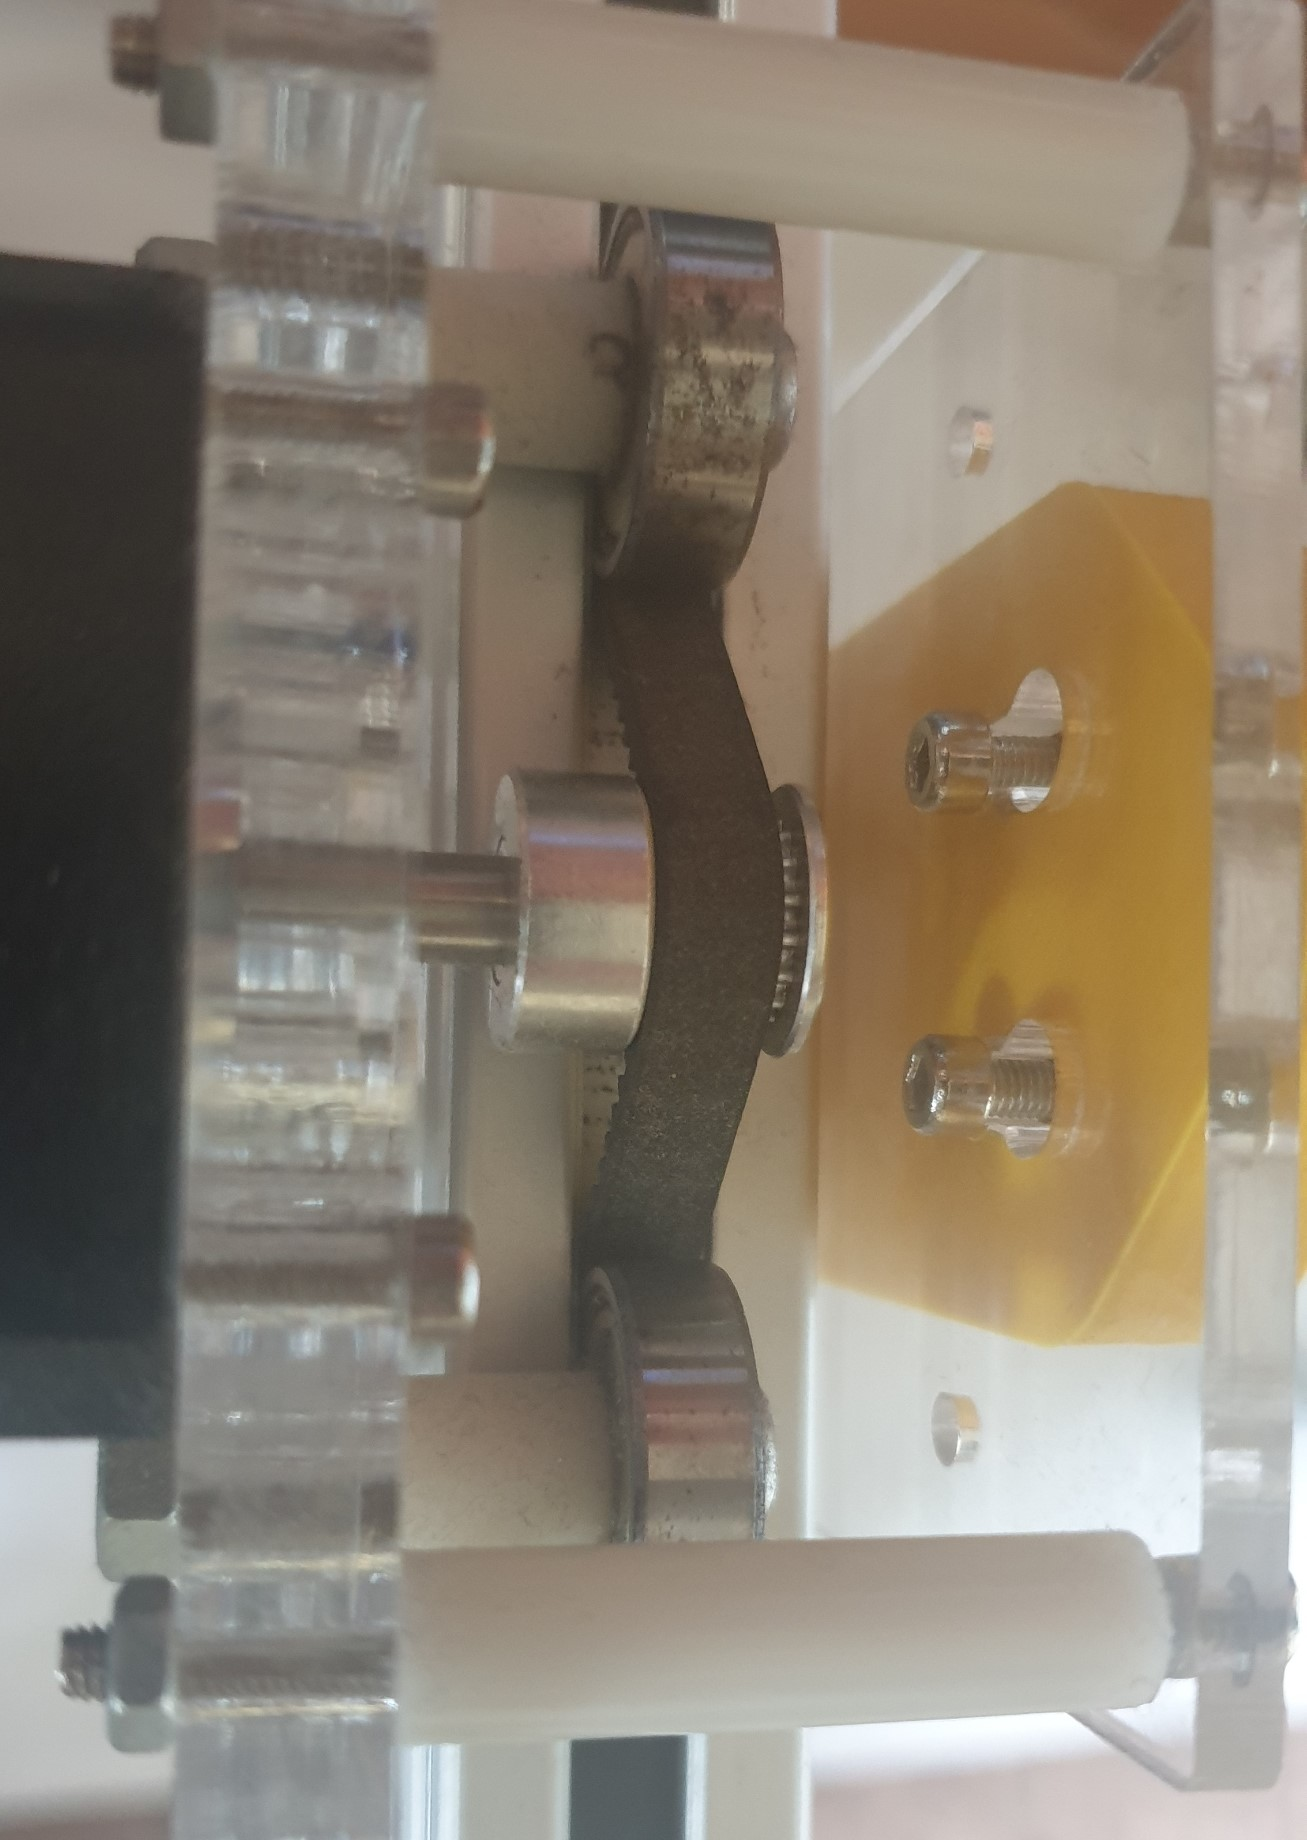
\includegraphics[height=5.5cm]{pages/dodatekARobot/img/przeniesienieNapeduW2.jpg}
	\end{subfigure}
	\begin{subfigure}{}
		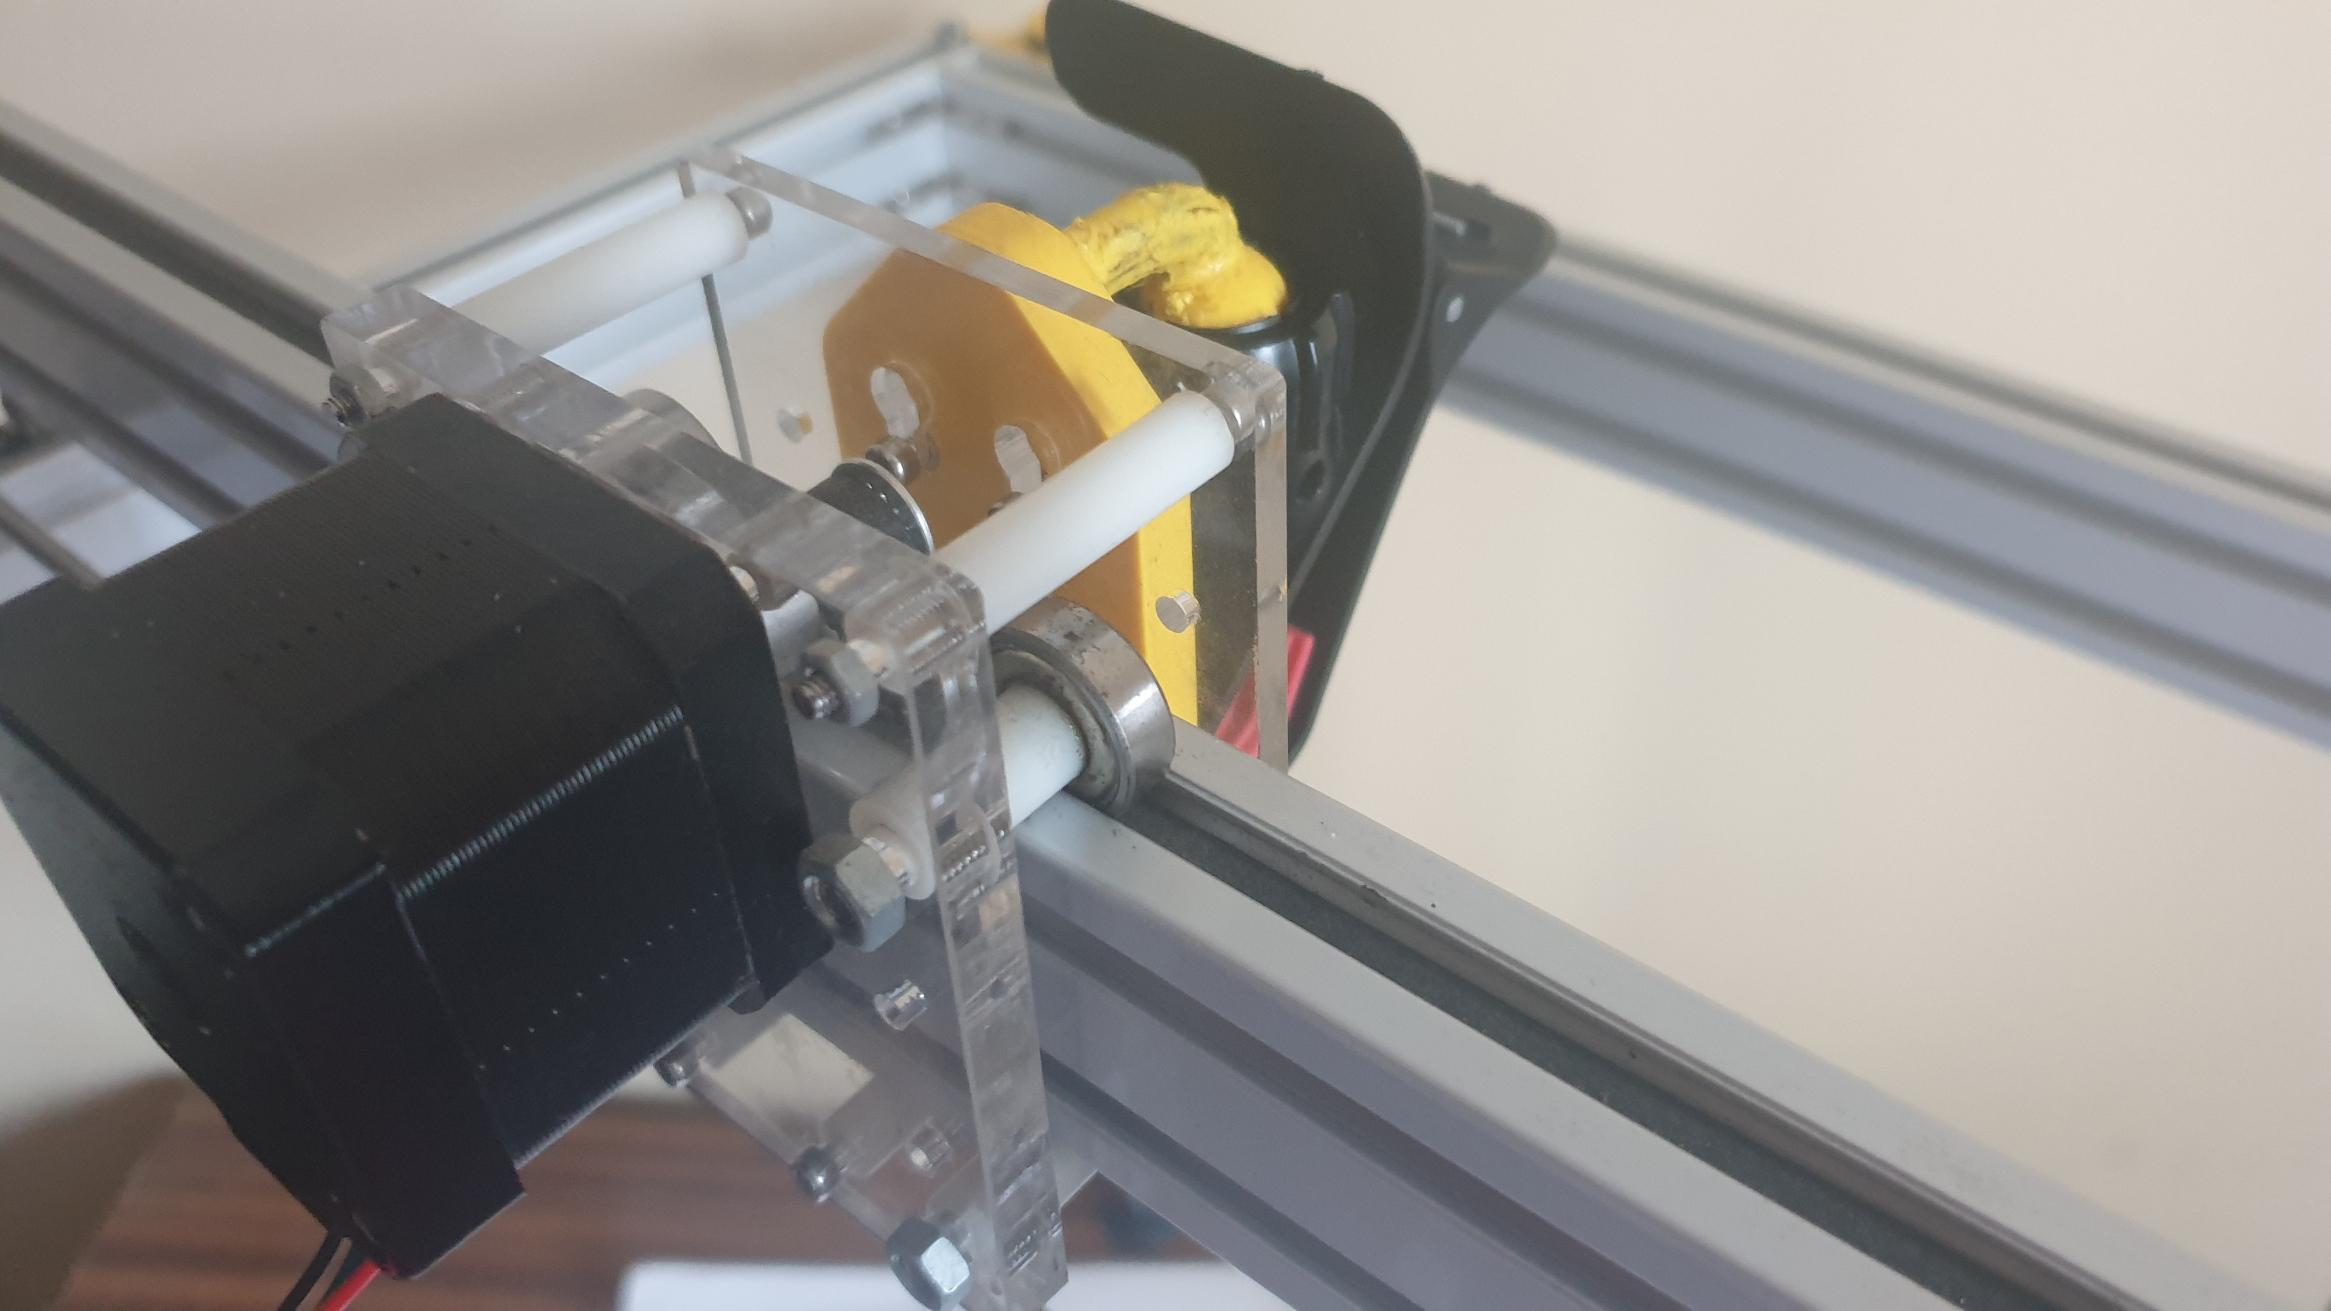
\includegraphics[height=5.5cm]{pages/dodatekARobot/img/widokNaOs2.jpg}
	\end{subfigure}
	\caption{Napęd osi przesuwającą karetką}
\end{figure}
Napęd drugiej osi został zrealizowany identycznie, poza tym że w tym przypadku koło zębate jest zamocowane bezpośrednio na osi silnika.

\textbf{Sterowanie i komunikacja} \newline
Sterowanie zrealizowane jest przy pomocy mikrokontrolera Arduino Nano i płytki z odpowiednimi sterownikami silników krokowych. 
Sterownik ma wgrany program pozwalający, na komunikacje z komputerem przy pomocy portu szeregowego i analizę wysyłanych komend G-Code.
Komendy pozwalają na poruszanie robotem z określoną prędkością lub modyfikacje parametrów pracy np. przejście z współrzędnych absolutnych na przyrostowe.

\begin{figure}[H]
	\centering
	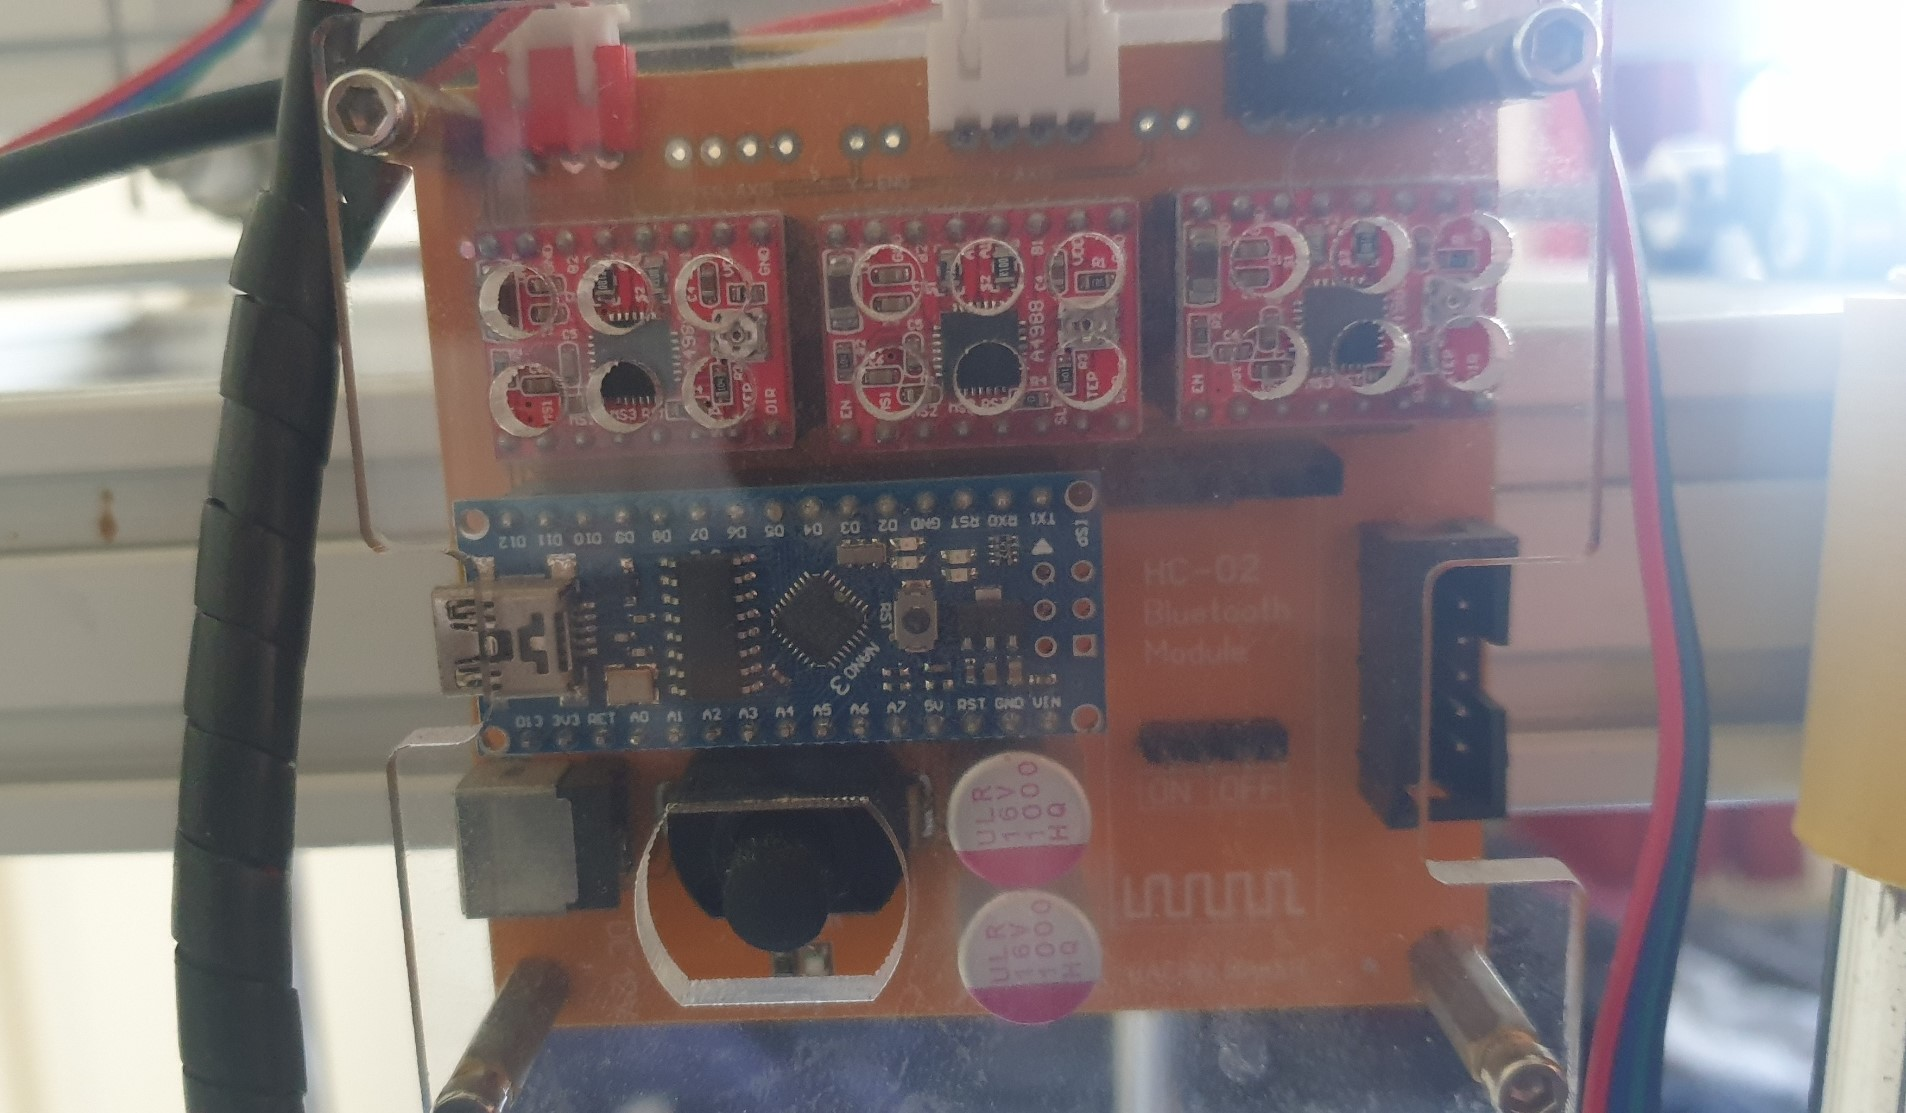
\includegraphics[width=0.70\linewidth]{pages/dodatekARobot/img/kontroler.jpg}
	\caption{Zdjęcie sterownika}
\end{figure}
Wykorzystano sterowniki silników krokowych opartych na układzie A4988. 
Modułowe sterowniki, pozwalają na szybką wymianę w przypadku awarii.

\textbf{Oprogramowanie sterownika} \newline
Do sterowania silnikami i interpretacji wysyłanych poleceń w formacie G-Code użyto otwartego projektu 
grbl\cite{grblGithub} w wersji 1.1f. Repozytorium z całym projektem można pobrać ze strony github. 
Dzięki zastosowaniu otwartego projektu, sterownik od razu zna wszystkie potrzebne komendy takie jak 
G0 (szybki ruch liniowy), G1 (ruch liniowy z narzędziem) czy inne jak G53 (zmiana systemu współrzędnych na absolutne).
Do uruchomienia projektu, potrzebujemy program Arduino IDE, które zawiera w sobie kompilator i potrzebny program programujący 
mikrokontroler sterownika. Przed kompilacją należy wskazać konkretne piny odpowiadające za sterowanie silnikami. 
Po wgraniu programu należy odpowiednio skonfigurować podstawowe parametry np. ilość kroków silnika potrzebną do przesunięcia się o 1mm. 
Ustawienia i zapisania parametrów dokonuje się poprzez wysłanie odpowiedniej kombinacji poleceń przy pomocy dowolnego 
terminala łączącego się poprzez port szeregowy np. PuTTy.

\textbf{Kamera} \newline
W tym przypadku jako kamerę wykorzystano telefon z zainstalowaną aplikacją iVCam. Aby połączyć się z komputera należy zainstalować 
program kliencki iVCam, który dodaje wirtualną kamerę do systemu. 
\begin{figure}[H]
	\begin{subfigure}{}
		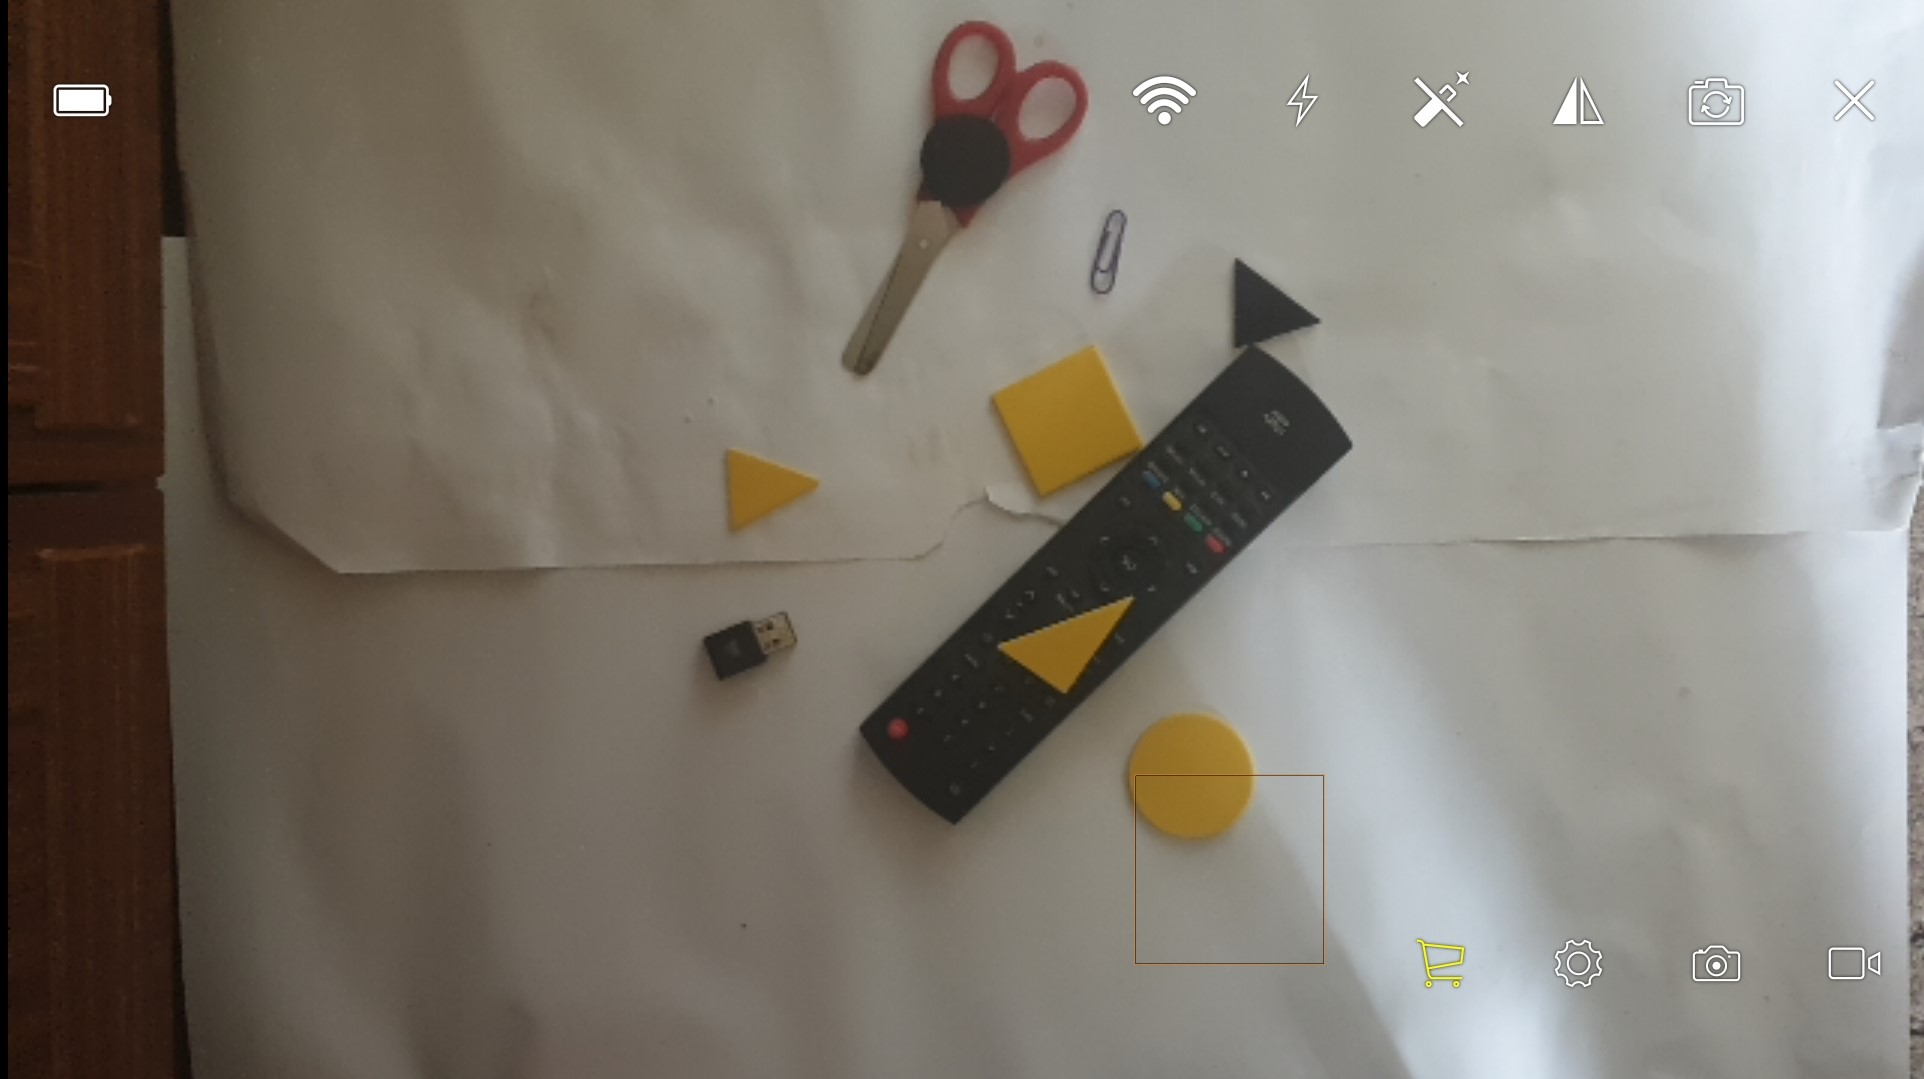
\includegraphics[height=4.5cm]{pages/dodatekARobot/img/kameraTelefon.jpg}
	\end{subfigure}
	\begin{subfigure}{}
		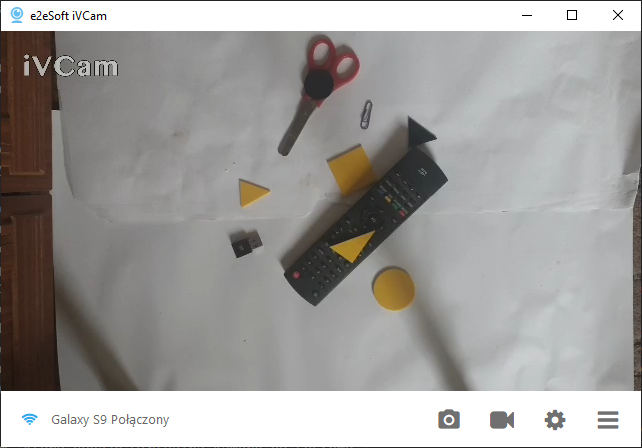
\includegraphics[height=4.5cm]{pages/dodatekARobot/img/kameraDesktop.png}
	\end{subfigure}
	\caption{Połączenie telefonu i komputera przy pomocy aplikacji iVCam}
\end{figure}

Jak widać na powyższym zdjęciu, telefon połączył się z aplikacją zainstalowana na komputerze. 
Aplikacja imituje zwykłą kamerę widoczną przez system operacyjny, dzięki czemu nie była potrzebna żadna dodatkowa 
biblioteka do obsługi połączenia bezprzewodowego. 
W porównaniu do wcześniej testowanym protokołem RTSP, to rozwiązanie cechuje się bardzo niskim opóźnieniem i dobrą jakością 
przesyłanego obrazu. Wadą aplikacji jest znak wodny z logiem, jednak nie przeszkadzał on w pracy sieci neuronowej. 

\section{Uczenie sieci neuronowej}
\subsection{Architektura algorytmu wykrywającego obiekty} \label{section:architekturaAlgorytmu}
Do zbudowania modelu wykrywającego wskazane klasy na zdjęciach użyto oprogramowania Matlab, dodatku
Deep Learning Toolbox oraz innych dodatków pozwalających na przetwarzanie obrazu. 
Wykorzystany model bazuje na sieci neuronowej nazwanej CSPDarkNet53 i wstępnie wytrenowanym na 
zbiorze \href{https://cocodataset.org/}{COCO} zawierającym ponad 200 tysięcy oznaczonych zdjęć i 80 różnych kategorii.
\begin{figure}[H]
	\centering
	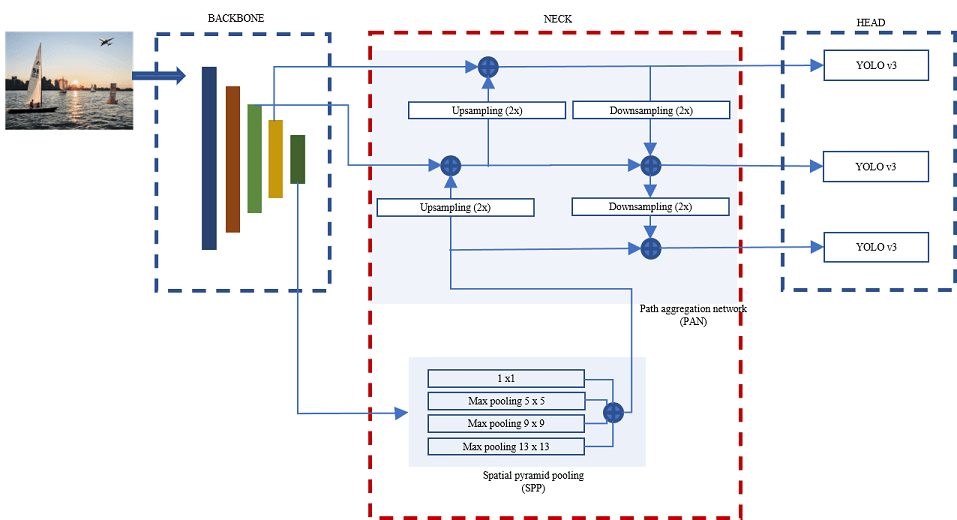
\includegraphics[width=12cm]{pages/uczenie/img/yolov4architecture.png}
	\caption{Sposób implementacji modelu YOLOv4 w Matlab'ie \cite{matlabOYolov4}}
	\label{fig:implementacjaWMatlabie}
\end{figure}
Implementacja algorytmu YOLO w Matlabie została podzielona na trzy różne sekcje. 
Pierwsza, oznaczona na rysunku \ref{fig:implementacjaWMatlabie} jako 'backbone', jest szkieletem sieci odpowiadającym za obliczenie 
mapy cech z obrazów wejściowych. Druga warstwa, łączy mapy cech z danymi z warstw sieci szkieletowej oraz wysyła je do kolejnego modułu.
Ostatni segment odpowiada za przetworzenie wcześniej wyodrębnionych cech, przewidzenie obwiedni i klasy obiektów.
\begin{figure}[H]
	\centering
	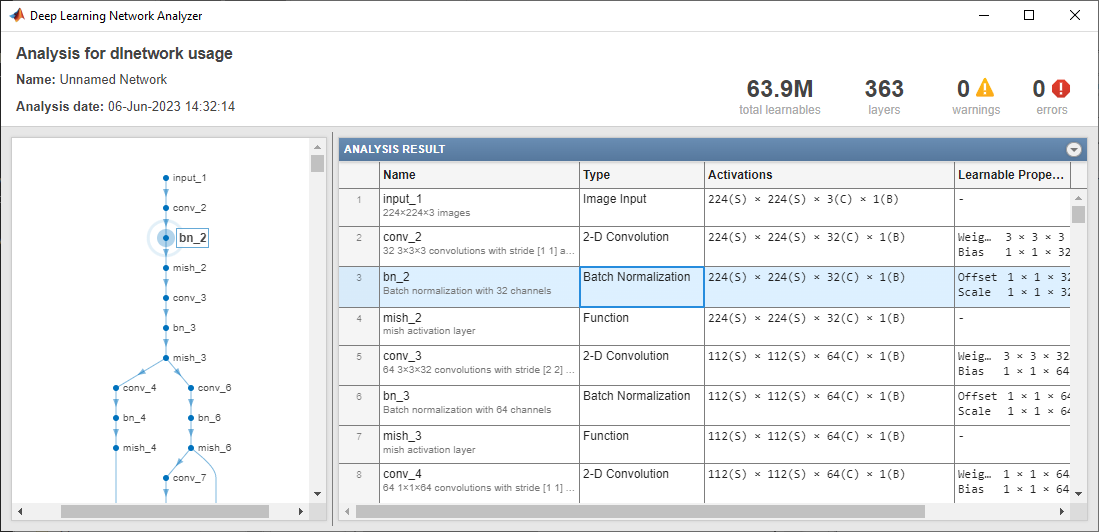
\includegraphics[width=10cm]{pages/uczenie/img/wielkoscSieciMatlabAnalyze.png}
	\caption{Parametry użytej sieci uzyskane funkcją analyzeNetwork}
\end{figure}

Użyta sieć składa się z 53 warstw konwolucyjnych, wejścia 224x224x3 oraz trzech 
wyjść określających prawdopodobieństwo występowania danej klasy. 
Cała sieć zbudowana jest z 363 warstw a do wyuczenia jest ponad 63mln parametrów.

Istnieje mniejsza sieć nazwana 'Tiny-YOLOv4', która posiada zaledwie około 30 warstw konwolucyjnych, dzięki czemu
została znacznie zwiększona szybkość działania, kosztem niewielkiego pomniejszenia skuteczności. 
Według wielu różnych źródeł wersja ta jest zdecydowanie lepsza do przetwarzania szybko zmieniającego się obrazu.
%========================================================
\subsection{Zbieranie danych}
\subsubsection{Automatyczne generowanie danych}
W pierwszej wersji dane miały być generowane przy pomocy automatycznego skryptu.
Utworzony program w Matlabie, otwierał wcześniej nagrany film z samym tłem, a następnie 
na pobranych klatkach obrazu wstawiał szablony z przygotowanymi obrazami docelowych obiektów.
Dzięki dynamicznemu generowaniu, można było zachować zróżnicowanie danych pomimo ich dużej ilości.

\begin{figure}[H]
	\centering
	\begin{minipage}{0.45\textwidth}
		\centering
		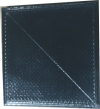
\includegraphics[width=3.5cm]{pages/uczenie/img/maska_kw3.png}
	\end{minipage}
	\begin{minipage}{0.45\textwidth}
		\centering
		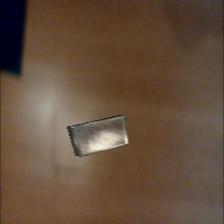
\includegraphics[width=3.5cm]{pages/uczenie/img/wynikGenerowania.jpg} % second figure itself
	\end{minipage}
	\caption{Lewe zdjęcie przedstawia maskę z usuniętym tłem a prawe klatkę nagranego filmu z naniesionym obiektem}
	\label{rys:przykladoweGenerowanieDanych}
\end{figure}

Jak widać na rysunku \ref{rys:przykladoweGenerowanieDanych}, generowane dane wyglądają dosyć sztucznie, głównie ze względu na 
tło oraz niekonsekwentne oświetlenie obiektu i tła. Ostatecznie wynikiem działania algorytmu był utworzony zbiór zdjęć
oraz jeden plik typu gTruth z zapisanymi obrazami, lokalizacją i klasą obiektów.
Poniżej dołączono skróconą wersje programu generującego zdjęcia.

\begin{lstlisting}[language=Matlab,caption=Generowanie danych]
	% automatyczne generowanie danych do uczenia sieci
	clc; clear;  close all;
	
	videoFiles = ["data/vid/w1.3gp", "data/vid/w2.3gp"];
	pathToSaveImages = "data/test2";
	outputImageSize = [224, 224];
	filterToOutputImage = fspecial("motion", 2, 2);
	
	dataKolo = {}; dataKwadrat = {}; dataTrojkat = {};
	dataFileNames = "";
	for vidName = videoFiles
		vid = VideoReader(vidName); %wczytanie filmu
		rrStep = int8(vid.NumFrames);
		for fIndX = 1 : 5 : vid.NumFrames % iteracja po klatkach
			frame = read(vid, fIndX);
	
			% dostosowanie klatki do rozmiaru sieci
			frame = imresize(frame, outputImageSize);
	
			% losowanie odpowiedniej maski/obiektu
			rr = randi([1, 6]);
			if(rr == 1) 
				[x, map, alpha] = imread("data\mask\kw_mask.png");
			% wczytywanie kolejnych masek
			end
			x = imresize(x, 0.5);
			alpha = imresize(alpha, 0.5);
			maskSize = size(x);        
			%wyznczenie pozycji 
			posX = randi([0, outputImageSize(1) - maskSize(1)]);
			posY = randi([0, outputImageSize(2) - maskSize(2)]);
	
			if(rr == 1 || rr == 2) % kwadrat
				dataKolo(end + 1) = {[]};
				dataKwadrat(end + 1) = {[posX, posY, maskSize(1), maskSize(2)]};
				dataTrojkat(end + 1) = {[]};
			elseif (rr == 5 || rr == 6 || rr > 5) % kolo
				dataKolo(end + 1) = {[posX, posY, maskSize(1), maskSize(2)]};
				dataKwadrat(end + 1) = {[]};
				dataTrojkat(end + 1) = {[]};
			elseif (rr == 3 || rr == 4) % tr
				dataKolo(end + 1) = {[]};
				dataKwadrat(end + 1) = {[]};
				dataTrojkat(end + 1) = {[posX, posY, maskSize(1), maskSize(2)]};
			end
	
			if (fIndX > rr * rrStep)
				rr = rr + 1;
			end
	
			% wzstawienie szablonu do obrazu
			frame = insertImageInPos(frame, x, alpha, posX, posY);
			% dodanie opcjonalnego filtru do zdjecia 
			if exist("filterToOutputImage" ,"var") == true
				frame = imfilter(frame, filterToOutputImage);
			end
	
			path = sprintf("%s/%i-%i.jpg", pathToSaveImages,randi(300), fIndX);
			dataFileNames = dataFileNames + path + ";";

			%zapisanie obrazu
			imwrite(frame, path)
		end
	end
	
	% zapisywanie danych jako obiektu datastore
	labels = labelDefinitionCreator();
	addLabel(labels, "kolo", "Rectangle");
	addLabel(labels, "kwadrat", "Rectangle");
	addLabel(labels, "trojkat", "Rectangle");
	labelData = table(dataKolo', dataKwadrat', dataTrojkat', 'VariableNames',{'kolo', 'kwadrat', 'trojkat'});
	
	t = split(dataFileNames, ";"); t(end) = [];
	f =  matlab.io.datastore.FileSet(t);
	imds = imageDatastore(f);
	labelDataStore = boxLabelDatastore(labelData);
	ds = combine(imds, labelDataStore);
	save("ds", "ds");
\end{lstlisting}
Skrypt otwierał wskazany film i pobierał co 5 klatkę obrazu. Dalej generowana była liczba określająca klasę wstawionego obiektu.
Szablon był wczytywany do pliku, a typ i losowo wygenerowana pozycja została zapisana w bazie danych.
Na końcu mógł zostać dodany filtr, mający poprawić efekt przejścia pomiędzy połączonymi obrazami. 
Tak przygotowane zdjęcie zostało zapisane na dysku. 
Po przetworzeniu filmu dane o obiektach, ich pozycjach oraz odpowiednich zdjęciach były zapisywane do odpowiedniego pliku.
\begin{figure}[H]
	\centering
	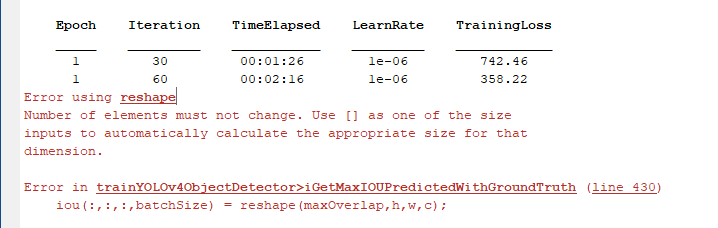
\includegraphics[width=12cm]{pages/uczenie/img/errorPrzyTrenowaniu.png}
	\caption{Błąd podczas trenowania obrazu}
\end{figure}
Ostatecznie największym problemem okazało się wytrenowanie sieci na tak wygenerowanych danych.
Prawdopodobnie algorytm źle zapisywał dane, ponieważ w trakcie trenowania pierwszej epoki i losowej iteracji trenowanie przerywało się,
wyświetlając komunikat z błędem funkcji 'reshape' wywoływanej wewnątrz funkcji trenującej model.

\subsubsection{Ręczne oznaczanie danych}
Docelowa i działająca sieć została wytrenowana na ręcznie oznaczonych zdjęciach. 
Dane zostały zebrane na wykonanym już robocie i nagrane poprzez symulowanie ruchów robota i przesuwanie docelowych obiektów.
Nagrane filmy zostały przetworzone poprzez skrypt, który pobrał z filmu co którąś klatkę a następnie przeskalował ją do docelowego rozmiaru. 


\begin{figure}[H]
	\centering
	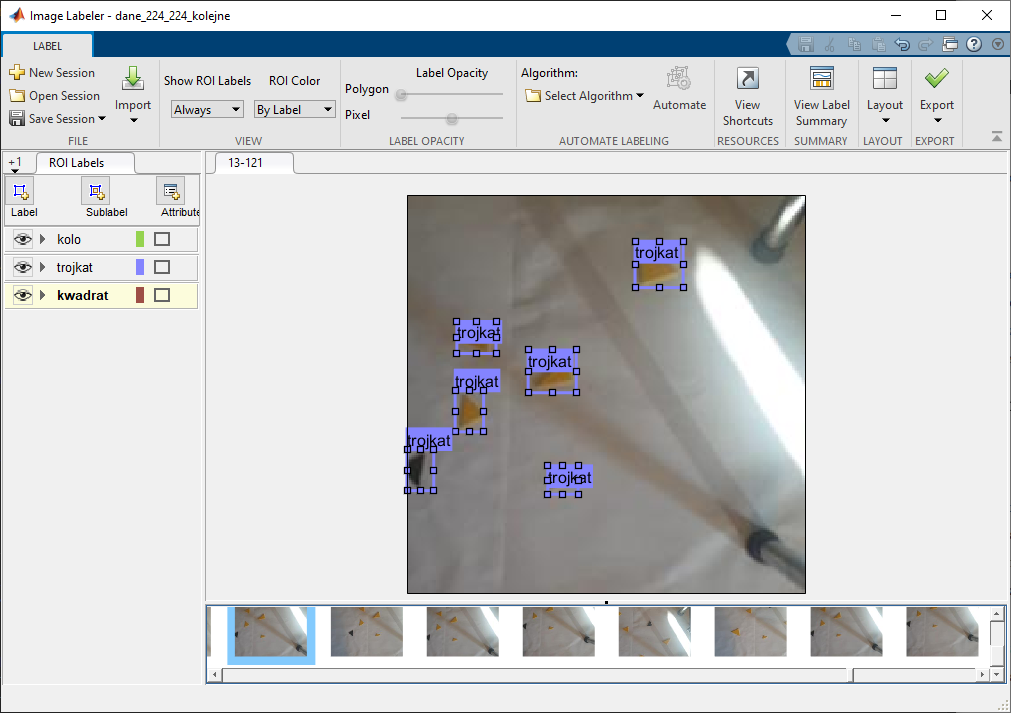
\includegraphics[width=12cm]{pages/uczenie/img/imageLabeler.png}
	\caption{Program imageLabeler, pozwalający na etykietowanie zdjęć}
	\label{fig:imgageLabelerMatlab}
\end{figure}
Rysunek \ref{fig:imgageLabelerMatlab} przedstawia zrzut ekranu programu, w którym zdefiniowano odpowiednie klasy, wczytano 
przygotowane dane oraz oznaczono odpowiednie obiekty ich klasami.
Baza zawiera ponad 1200 zdjęć z obiektami (zmienione orientacje, pozycje, kształt) i różnym tłem (zmiana oświetlenia, dodatkowe cienie).

\begin{figure}[H]
	\centering
	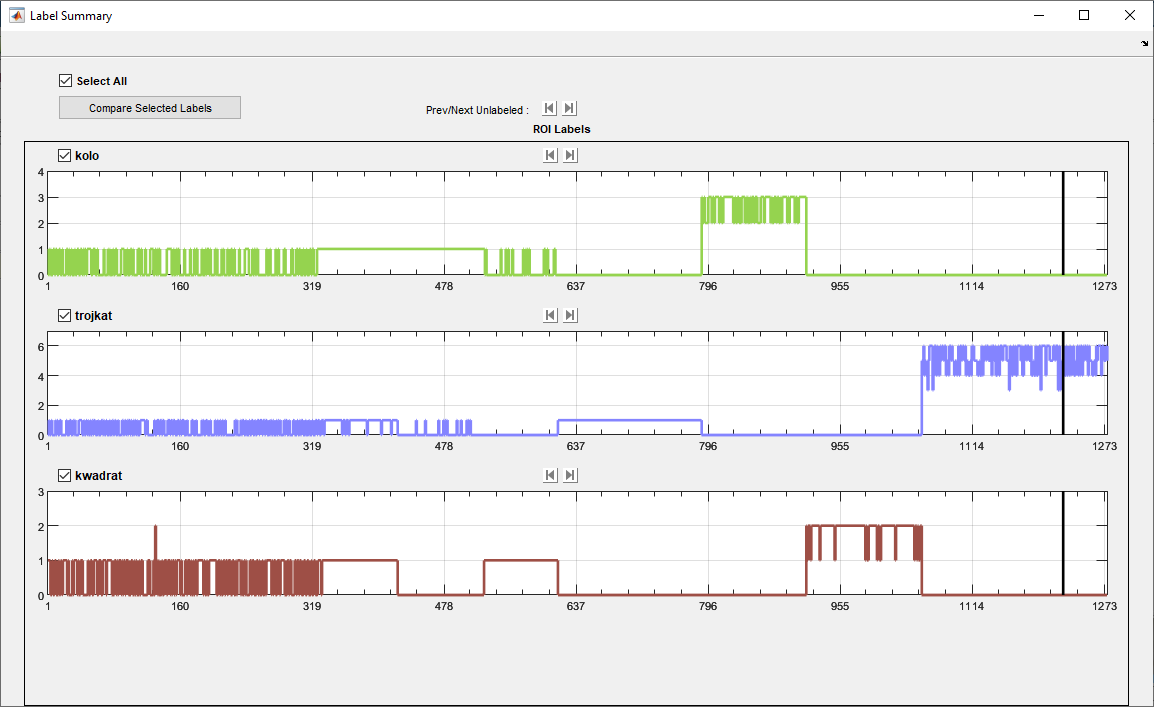
\includegraphics[width=14cm]{pages/uczenie/img/podsumowanieRozkladuEtykiet.png}
	\caption{Rozkład klas w poszczególnych zdjęciach}
\end{figure}
Baza zdjęć była systematycznie zwiększana wraz z analizą skuteczności działania wytrenowanej sieci. 
Jak widać najwięcej jest zdjęć zawierających kwadraty, a najmniej, ze względu na uniwersalny kształt, kół. 
Ostatecznie rozkład klas prezentuje się następująco: 
\begin{figure}[H]
	\centering
	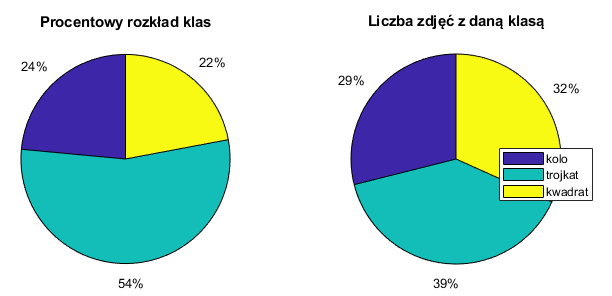
\includegraphics[width=16cm]{pages/uczenie/img/rozkladKlas.png}
	\caption{Ogólny rozkład klas}
\end{figure}
Jak widać zgodnie z oczekiwaniami w bazie ze względu na największą ilość konfiguracji jest najwięcej zdjęć trójkątów. 
Liczba kół i kwadratów jest bardzo podobna. 
Poniżej został zaprezentowane przykładowe zdjęcia. 
\begin{figure}[H]
	\centering
	\begin{minipage}{0.30\textwidth}
		\centering
		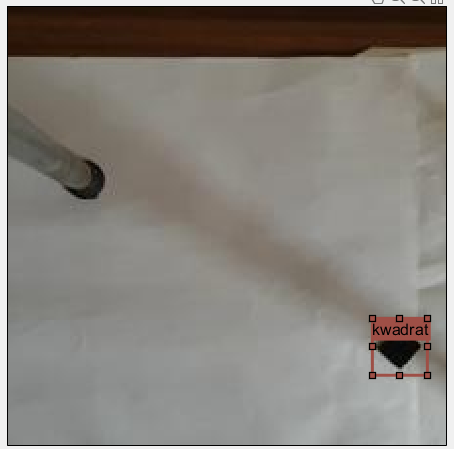
\includegraphics[width=4.5cm]{pages/uczenie/img/przykladoweDaneV1.png} % first figure itself
	\end{minipage}\hfill
	\begin{minipage}{0.3\textwidth}
		\centering
		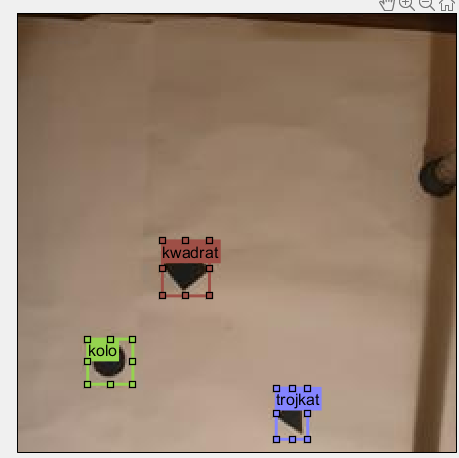
\includegraphics[width=4.5cm]{pages/uczenie/img/przykladoweDaneV2.png} % second figure itself
	\end{minipage}\hfill
	\begin{minipage}{0.3\textwidth}
		\centering
		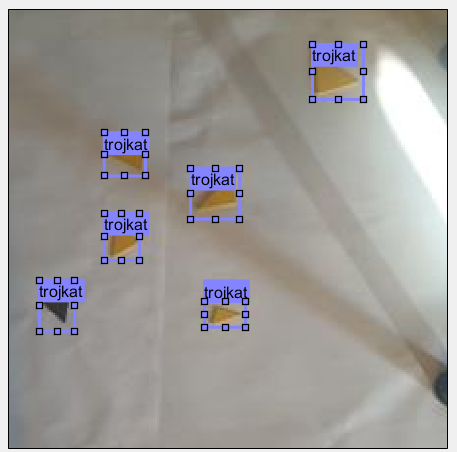
\includegraphics[width=4.5cm]{pages/uczenie/img/przykladoweDaneV3.png} % second figure itself
	\end{minipage}
						
	\caption{Przykładowe otagowane zdjęcia}
\end{figure}
Pierwsze fotografie zawierają pojedyncze obiekty, jednak wraz z rozwojem, na zdjęciach pojawiało się coraz więcej różnych obiektów.
%========================================================
\subsection{Uczenie sieci}
Sieć neuronowa była trenowana przy pomocy toolbox'a Deep Learning Toolbox w Matlabie, przy pomocy poniższego skryptu.
% \begin{lstlisting}[language=Matlab,caption=Uczenie sieci]

% \end{lstlisting}
\lstinputlisting[language=Matlab,caption=Uczenie sieci]{pages/uczenie/skryptUczenie.txt}


Ze względu na małą ilość pamięci graficznej, uczenie odbywa się na procesorze. 
Podczas jednej iteracji, algorytm przetwarza jednocześnie 16 zdjęć (parametr MiniBatchSize). Przy takiej konfiguracji, uczenie 
na GPU nie było możliwe, a jednocześnie po zmniejszeniu tego parametru do 1 uczenie nie było tak skuteczne jak w przypadku jednoczesnego 
przetwarzania większej ilości obrazów.
Parametry uczenia sieci:
\begin{itemize}
	\item metoda uczenia: sgdm (Stochastic Gradient Descent with momentum),
	\item współczynnik uczenia: 0.001,
	\item liczba epok: 20.
\end{itemize}
Ostatecznie finalny model był douczany przy pomocy powyższego skryptu trzy razy co oznacza, że przeszedł przez 60 epok. 
Zbyt duża ilość epok uczących sieć może spowodować negatywny wynik z powodu przetrenowania sieci i ścisłego dopasowania się do danych treningowych.
\begin{figure}[H]
	\centering
	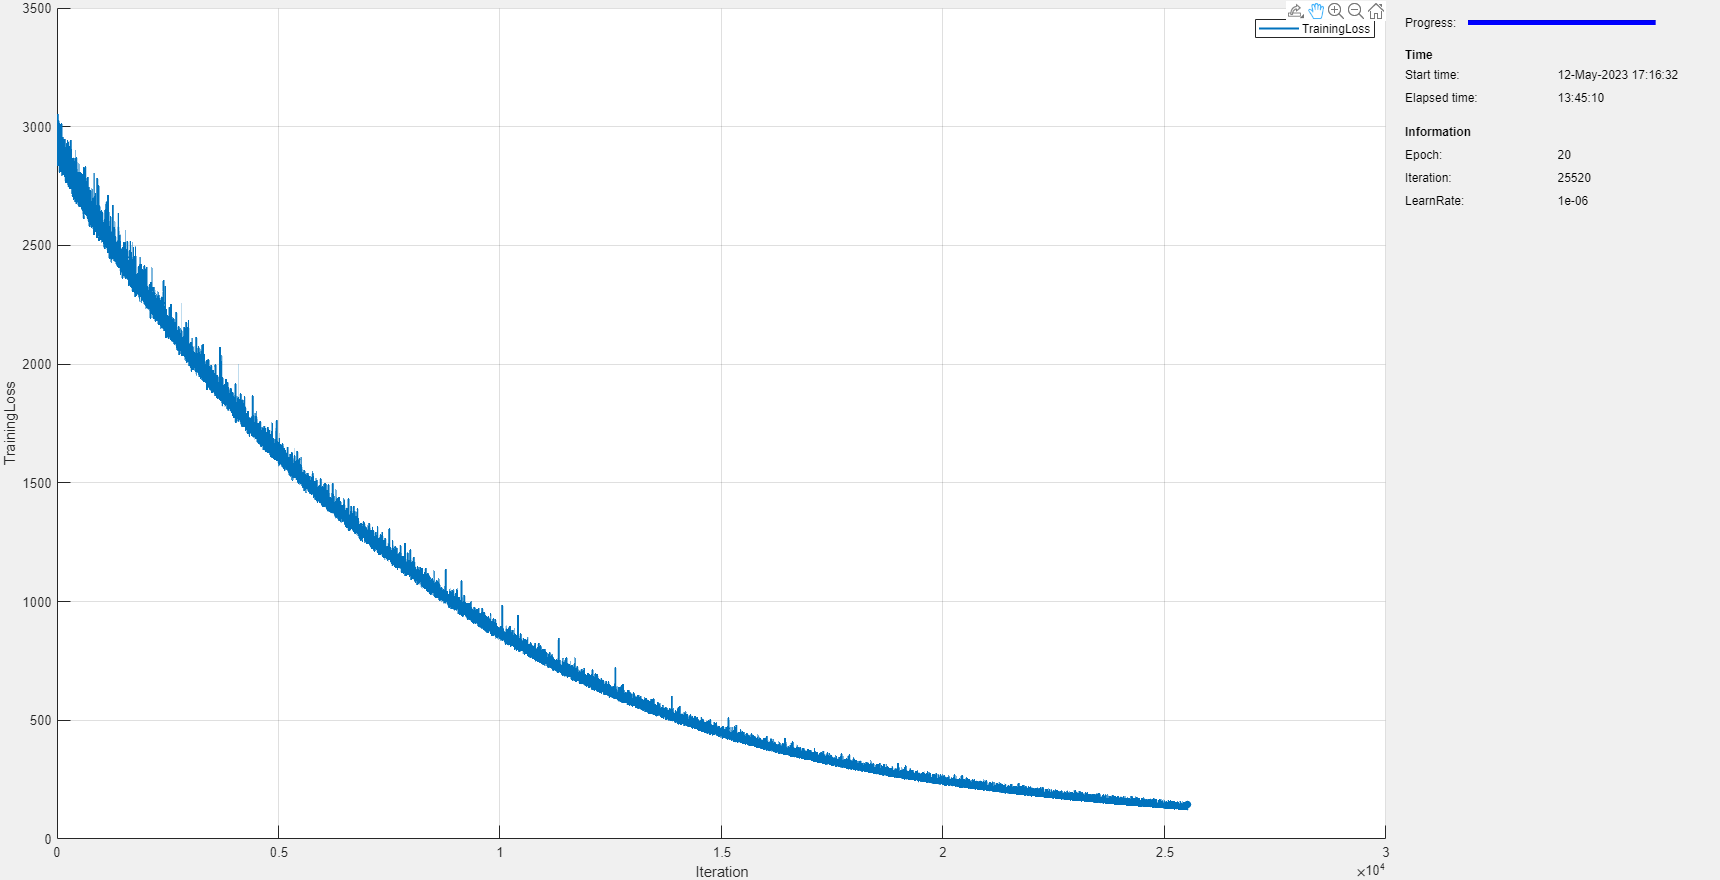
\includegraphics[width=14cm]{pages/uczenie/img/wykresTrenowanie.png}
	\caption{Przebieg błędu w zależności od liczby epok}
	\label{fig:bladWUczeniu}
\end{figure}
Wykres z rysunku \ref{fig:bladWUczeniu}, przedstawia przebieg trenowania i spadku błędu. Widać, że na początku procesu błąd bardzo szybko spada, 
jednak od połowy uczenia tendencja spada. Zdjęcie pochodzi z pierwszego etapu trenowania, gdzie trenowanie było efektywniejsze. 
Kolejne dwa etapy trenowania cechowały się spadkiem z około 50 do 0,2 wartości błędu. 

\subsection{Testy}
Aby sprawdzić skuteczność sieci, przeprowadzono testy polegające na podaniu wcześniej
niewidzianego obrazu z wieloma obiektami, 
ręczne przeanalizowanie wyników sieci i porównanie ich z rzeczywistą liczbą obiektów.
\begin{figure}[H]
	\centering
	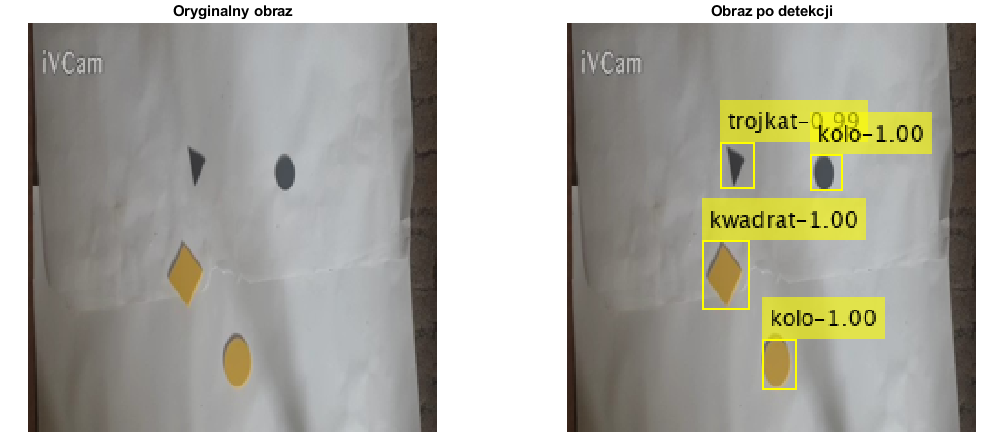
\includegraphics[width=15cm]{pages/uczenie/img/testyWynikSieci1.png}
	\caption{Pierwszy test z dobrym oświetleniem}
	\label{fig:testSieci1}
\end{figure}
Na podstawie wyniku pokazanemu na rysunku \ref{fig:testSieci1} widać, że sieć w sprzyjających warunkach radzi sobie z rozpoznawaniem różnych obiektów,
leżących w różnych orientacjach i pozycjach. Równocześnie należy zwrócić uwagę na bardzo duże wskaźniki pewności sieci wykrytych obiektów. 
\begin{figure}[H]
	\centering
	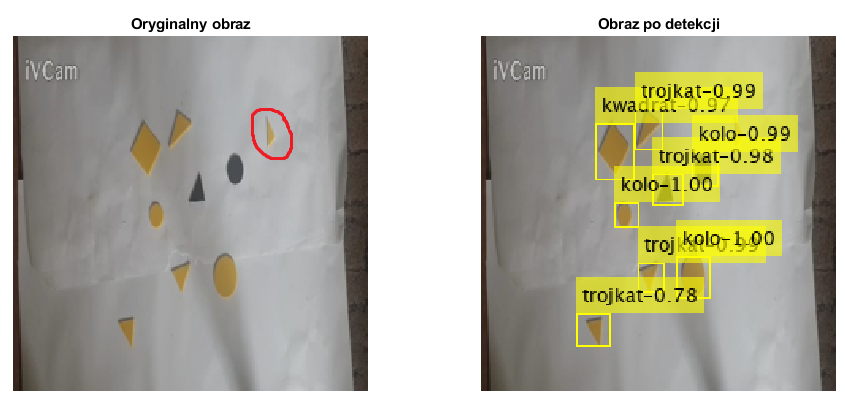
\includegraphics[width=15cm]{pages/uczenie/img/testyWynikSieci2.png}
	\caption{Test z dużą ilością różnych obiektów}
	\label{fig:testSieci2}
\end{figure}
Analizując przypadek przy dobrym oświetleniu z rysunku \ref{fig:testSieci2}, widać, że sieć ogólnie dobrze poradziła sobie z tak dużą liczbą różnych obiektów. 
Analizując dokładniej obraz, można zauważyć, że nie wykryty został jeden mniejszy trójkąt (zaznaczony na czerwono).
\begin{figure}[H]
	\centering
	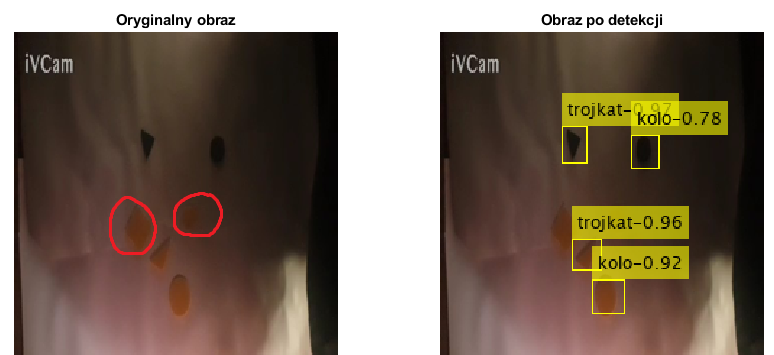
\includegraphics[width=15cm]{pages/uczenie/img/testyWynikSieci3SlabeOsw.png}
	\caption{Test przy słabym oświetleniu}
	\label{fig:testSieci3}
\end{figure}
Po ograniczeniu światła sieć rozpoznała tylko cztery z sześciu obiektów. 
Równocześnie w porównaniu do poprzednich eksperymentów spadły wskaźniki pewności.
Należy zauważyć, że pominięte obiekty są bardzo słabo widoczne i w pierwszej chwili
nawet ludzkie oko może mieć problem z szybką lokalizacją.
\begin{figure}[H]
	\centering
	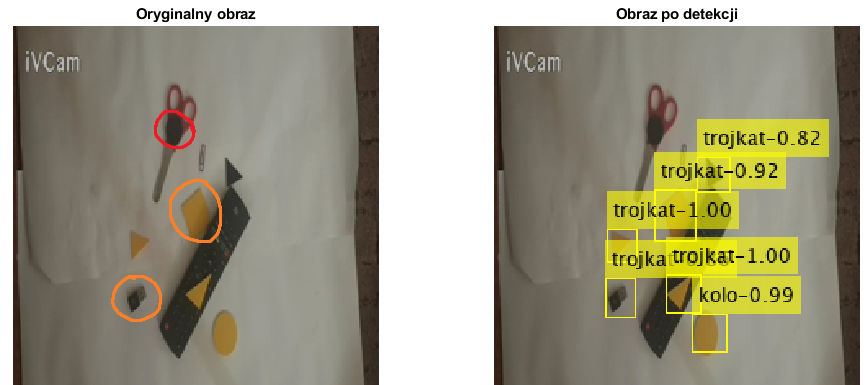
\includegraphics[width=15cm]{pages/uczenie/img/testyWynikSieci4.png}
	\caption{Testy z nieznanymi obiektami}
\end{figure}
Ostatni test został przeprowadzony po dodaniu nieznanych sieci obiektów.
Widać, że sieć nie rozpoznała leżącego na nożyczkach koła i 
źle sklasyfikowała dwa obiekty (oznaczone pomarańczową otoczką). Żółty kwadrat i leżący niżej moduł do myszki bezprzewodowej 
oznaczyła jako trójkąt. Podobnie jak w poprzednim przypadku, przy tak niskiej rozdzielczości trudno jest 
ludzkim okiem rozpoznać, że nie jest to żaden z wytrenowanych obiektów, choć ten bardziej przypomina kwadrat, a nie trójkąt.


\section{Połączenie systemów}
\begin{figure}[H]
	\centering
	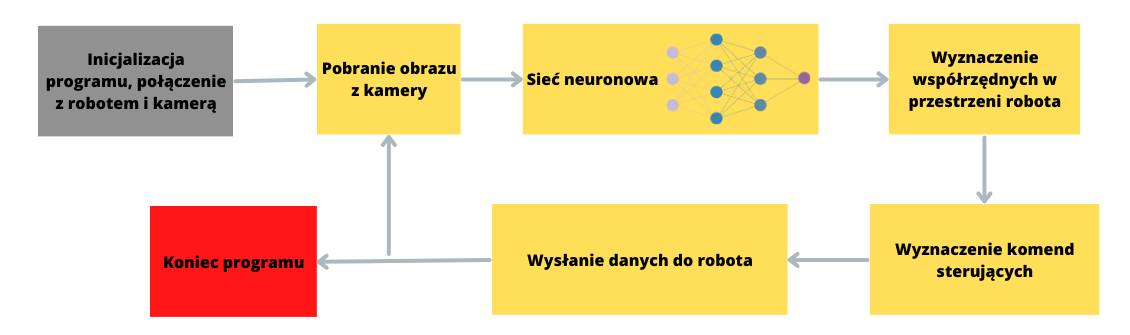
\includegraphics[width=16cm]{pages/siecIRobot/zdjecia/schematAlgorytmu.png}
	\caption{Ogólny schemat działania algorytmu}
	\label{rys:algorytmSterowania}
\end{figure}
Jak widać na algorytmie sterowania z rysunku \ref{rys:algorytmSterowania}, program w pierwszej kolejności inicjalizuje potrzebne komponenty
takie jak: kamera, połączenie z robotem oraz wczytanie wybranego modelu sieci neuronowej.
Po uruchomieniu głównej pętli algorytmu, pobierany jest obraz z kamery, który przekazywany jest do sieci neuronowej realizującej 
detekcję obiektów. Po wykryciu obiektów, wybierany jest docelowy, a następnie na podstawie jego pozycji wyznaczana jest komenda odpowiadająca 
za przesunięcie karetki robota. Cały proces jest zapętlony aż do momentu zatrzymania przez użytkownika. 
\subsection{Wykonana aplikacja kliencka}
Program obsługujący komunikacje z robotem i kamerą oraz uruchomienie sieci neuronowej wykonano w Matlab'ie i dodatku AppDesigner, 
który pozwala na zbudowanie graficznego interfejsu użytkownika i uruchamianie wytrenowanych modułów z siecią neuronową. 
\begin{figure}[H]
	\centering
	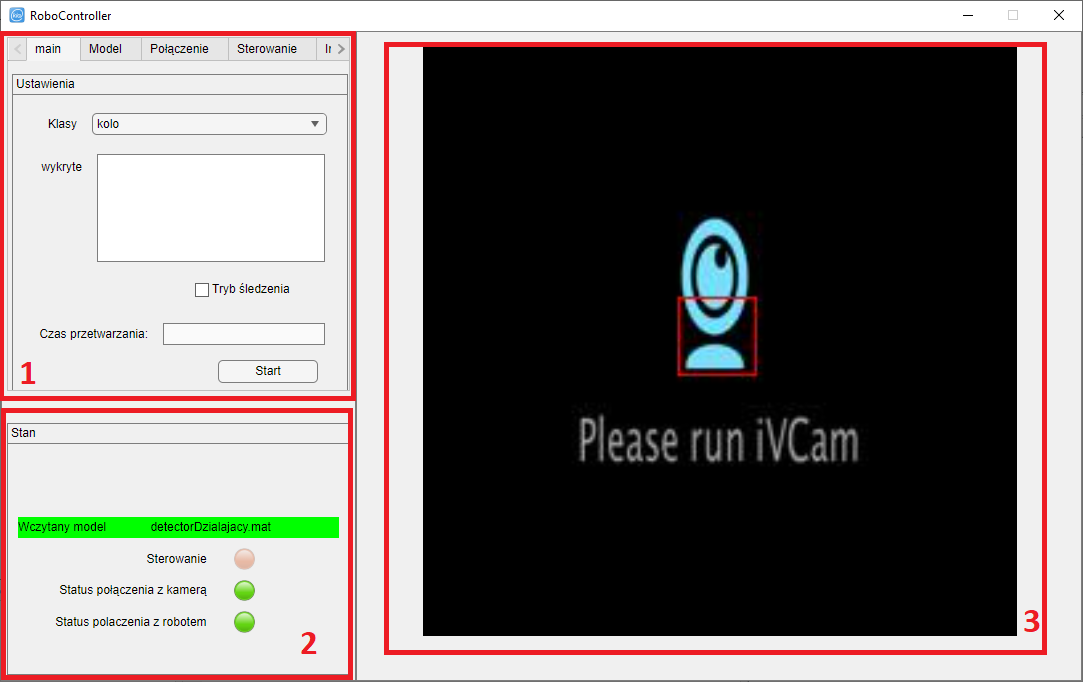
\includegraphics[width=12cm]{pages/siecIRobot/zdjecia/program/programCaly.png}
	\caption{Widok wykonanego programu}
	\label{fig:schematSterujacy}
\end{figure}
Na rys. \ref{fig:schematSterujacy} widoczne jest główne okno aplikacji. Możemy wyróżnić trzy odrębne sekcje,
odpowiadające kolejno za ustawienia sterowania, podgląd stanu poszczególnych modułów oraz podgląd obrazu i nałożonych na niego wyników sieci.
\begin{figure}[H]
	\centering
	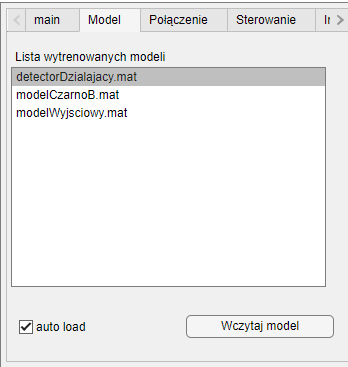
\includegraphics[height=4.5cm]{pages/siecIRobot/zdjecia/program/programUstModel.png}
	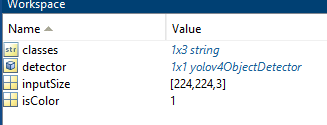
\includegraphics[height=4cm]{pages/siecIRobot/zdjecia/program/daneModeluSieci.png}
	\caption{Wczytanie danych modelu i jego struktura}
\end{figure}
Program pozwala na wczytanie wybranego pliku z modelem i jego ustawieniami. Opcja 'auto load' oznacza,
że model zostanie wczytany automatycznie zaraz po uruchomieniu aplikacji co przyśpieszyło proces testowania programu. 
Plik przechowuje wytrenowaną sieć neuronową i waży około 233Mb co oznacza, że ładowanie powoduje znaczne spowolnienie programu przy starcie.
\begin{figure}[H]
	\centering
	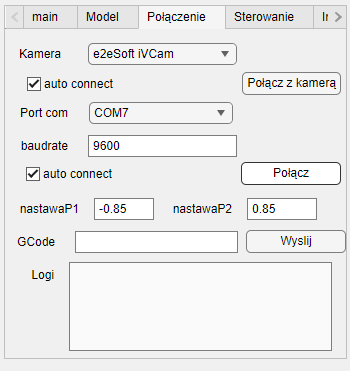
\includegraphics[height=6.5cm]{pages/siecIRobot/zdjecia/program/programUstPolaczenie.png}
	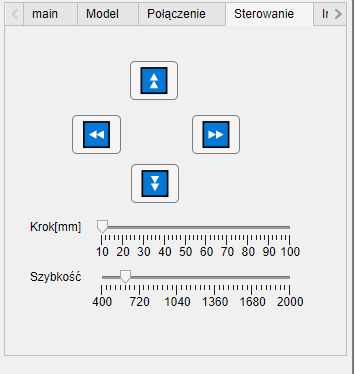
\includegraphics[height=6.5cm]{pages/siecIRobot/zdjecia/program/programUstSterowanie.png}
	\caption{Ustawienia połączeń oraz ręczne sterowanie robotem}
\end{figure}
Lewy zrzut ekranu przedstawia zakładkę pozwalającą na ustawienia połączenia pomiędzy aplikacją, a robotem i kamerą. 
Po połączeniu użytkownik ma możliwość wysłania własnej komendy G-Code wprowadzonej w odpowiednim polu. 
Dane odebrane po wysłaniu polecenia wyświetlane są w polu logów. Ekran z prawej strony po wybraniu prędkości i przesunięcia
pozwala na ręczne sterowanie karetką robota.
\begin{figure}[H]
	\centering
	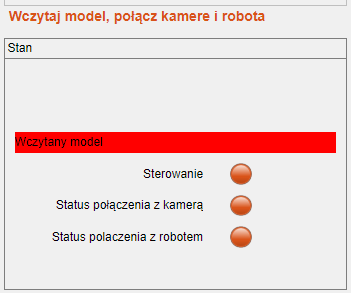
\includegraphics[height=6cm]{pages/siecIRobot/zdjecia/program/programStanErr.png}
	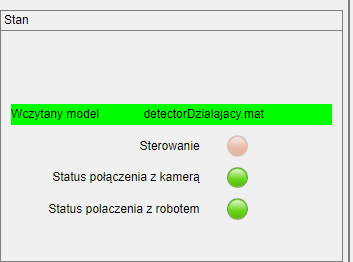
\includegraphics[height=6cm]{pages/siecIRobot/zdjecia/program/programStan.png}
	\caption{Stan aplikacji}
\end{figure}
Stan aplikacji jest cały czas prezentowany przy pomocy prostych kontrolek zmieniających swój kolor. 
Wczytanie modelu z siecią sygnalizowane jest poprzez zielony kolor i nazwę wczytanego pliku. 
Podobnie poprzez kolor sygnalizowany jest stan połączenia z robotem i zamocowaną na nim kamerą.
Kontrolka 'Sterowanie' informuje o tym, czy uruchomiony jest algorytm śledzący wybrany obiekt. 
Ostatecznie aplikacja została skompilowana do wykonywalnego pliku exe, który można uruchomić na dowolnym komputerze.
\subsection{Generowanie komend i sterowanie robotem}
Program posiada dwa różne tryby sterowania. Pierwszy tryb, po uruchomieniu algorytmu szuka wybranego obiektu, a po 
jego znalezieniu wyznacza różnicę pomiędzy środkiem obrazu, a zaznaczoną ramką i jednorazowo wysyła komendę G-Code.
Tryb "śledzenia", w przeciwieństwie do poprzedniego cały czas uruchamia sieć neuronową rozpoznającą obiekty i
wyznacza komendy odpowiadające za niewielkie przesunięcia. 
Tryb ten nazwany jest śledzącym, ponieważ dynamicznie reaguje na zmianę pozycji danego obiektu i stale za nim podąża.
\lstinputlisting[language=Matlab,caption=Uczenie sieci, label=kod:listingAlgorytmu]{pages/siecIRobot/kodSkryptu.m}
Program z listingu \ref{kod:listingAlgorytmu}, odpowiada za algorytm śledzący obiekty znalezione przez sieć neuronową. 
Niezależnie od trybu śledzenia wywoływana jest funkcja mainLoop, która odpowiada za pobranie
obrazu z kamery, uruchomienie odpowiedniej wersji algorytmu oraz dodanie do finalnego obrazu 'celownika', 
dodającego punkt odniesienia względem środka. W przypadku prostszej wersji, uruchamiana jest detekcja obiektów przy pomocy 
sieci neuronowej aż do momentu wykrycia pożądanej klasy. Po wykryciu obiektu algorytm wyznacza potrzebne do osiągnięcia celu przesunięcie, 
a następnie odpowiednio przygotowane polecenie wysyła do robota. Przesunięcie wyznaczane jest na podstawie różnicy 
środka obrazu i wykrytego obiektu, ten błąd dalej wzmacniany jest poprzez odpowiednie nastawy P1 i P2. 
Jak widać jest to regulator typu P, a współczynniki wzmocnień proporcjonalnych odzwierciedlają skalę pomiędzy obrazem, a rzeczywistą odległością.
Tryb śledzenia różni się tym, że sieć neuronowa uruchamiana jest ciągle i dzięki temu robot może nieustannie korygować błąd nadążania. 
Poza tym wyznaczone maksymalne przesunięcie ograniczone jest do stałej wartości tak, aby robot nie wykonywał zbyt dużych niepotrzebnych ruchów. 

\section{Przeprowadzone testy}
\subsection{Testowanie trybu normalnego}
Jako pierwsze wykonano testy trybu jednorazowo ustawiającego się nad wybranym obiektem. Aby uruchomić ten tryb, należy wpierw 
połączyć się z robotem i kamerą, wczytać wybrany model, a następnie w głównej zakładce wybrać docelowy obiekt. 
Po tym trzeba nacisnąć przycisk start i algorytm będzie zapętlony do momentu wykrycia pierwszego obiektu i wygenerowania komendy 
przesuwającej uchwyt z kamerą. 
\begin{figure}[H]
	\centering
	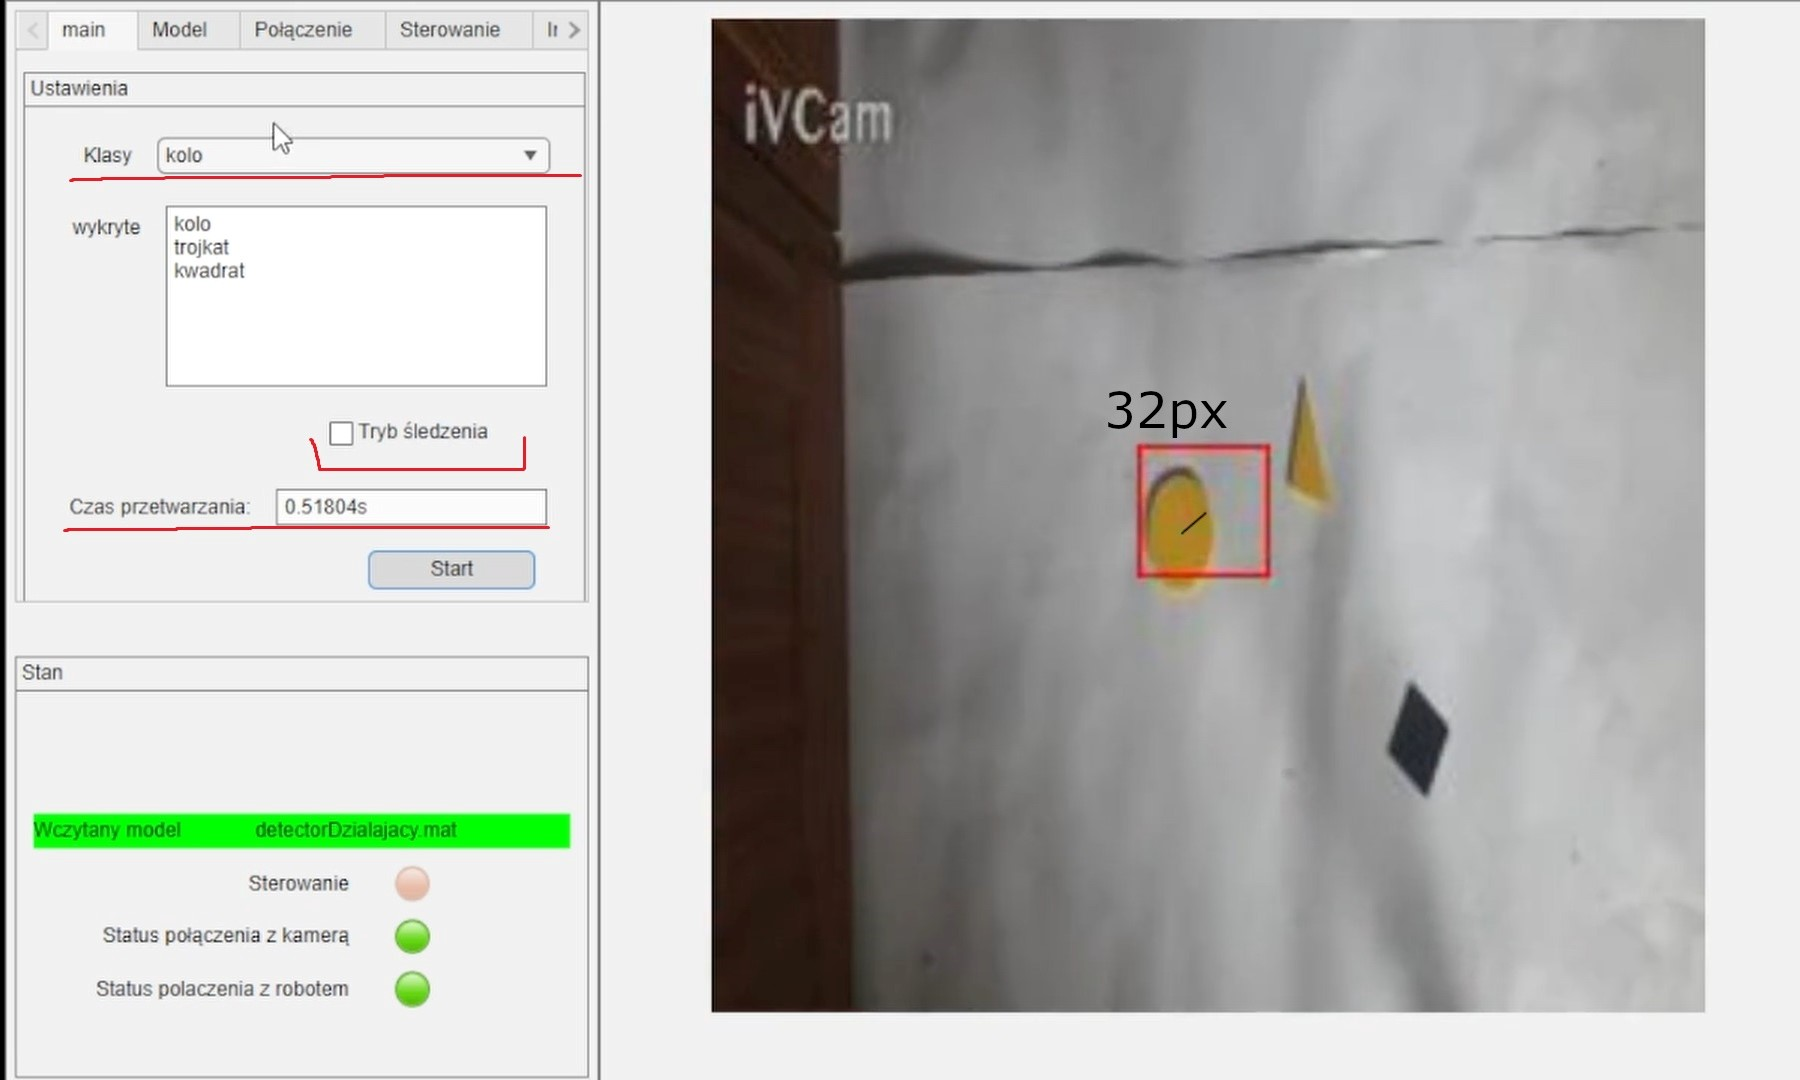
\includegraphics[width=14cm]{pages/testy/img/test1_1.jpg}
	\caption{Test trybu normalnego - wyśledzenie koła}
	\label{rys:testTrybuNormalnego1}
\end{figure}
Na rysunku \ref{rys:testTrybuNormalnego1} widać, że sieć wykryła koło a następnie wygenerowała komendę, która spowodowała przesunięcie. 
Oznaczony został element interfejsu użytkownika, pozwalający na wybranie docelowego obiektu oraz wyświetlający wszystkie znalezione na zdjęciu klasy.
W celu określenia błędu pomiędzy środkiem obrazu a osiągniętą pozycją, dodana została czarna linia. W powyższym przykładzie widać, 
że linia ta ma 32 pixele, a koło znajduję się w 'celowniku', jednak ich środki nie pokrywają się.
\begin{figure}[H]
	\centering
	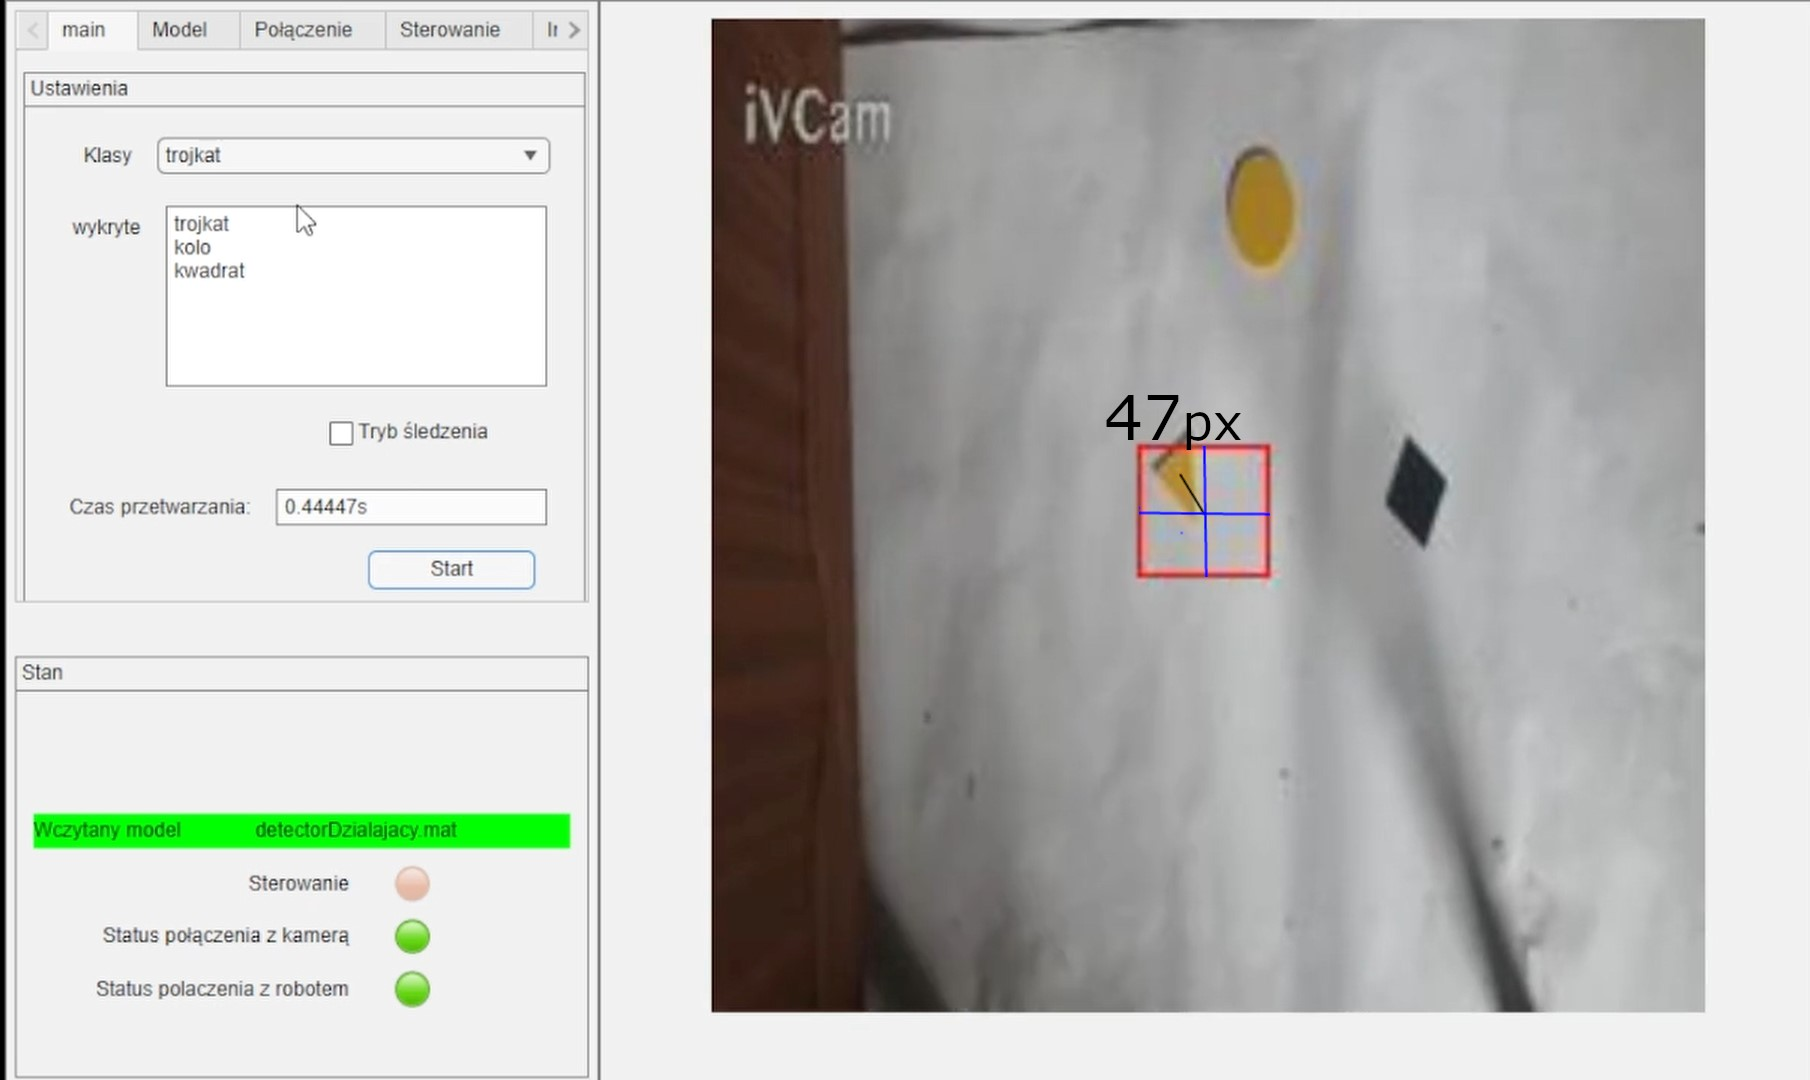
\includegraphics[width=14cm]{pages/testy/img/test1_2.jpg}
	\caption{Test trybu normalnego - znalezienie trójkąta}
\end{figure}
Przed uruchomieniem kolejnego testu, zmieniono pozycje obiektów i wybraną w programie kategorie. 
Sieć neuronowa znalazła wszystkie obiekty na obrazie, ale również w tym przypadku ostateczna pozycja cechowała się 
dużym błędem względem środków. Widać, że nawet w porównaniu do poprzedniego przypadku błąd ten wzrósł.
\begin{figure}[H]
	\centering
	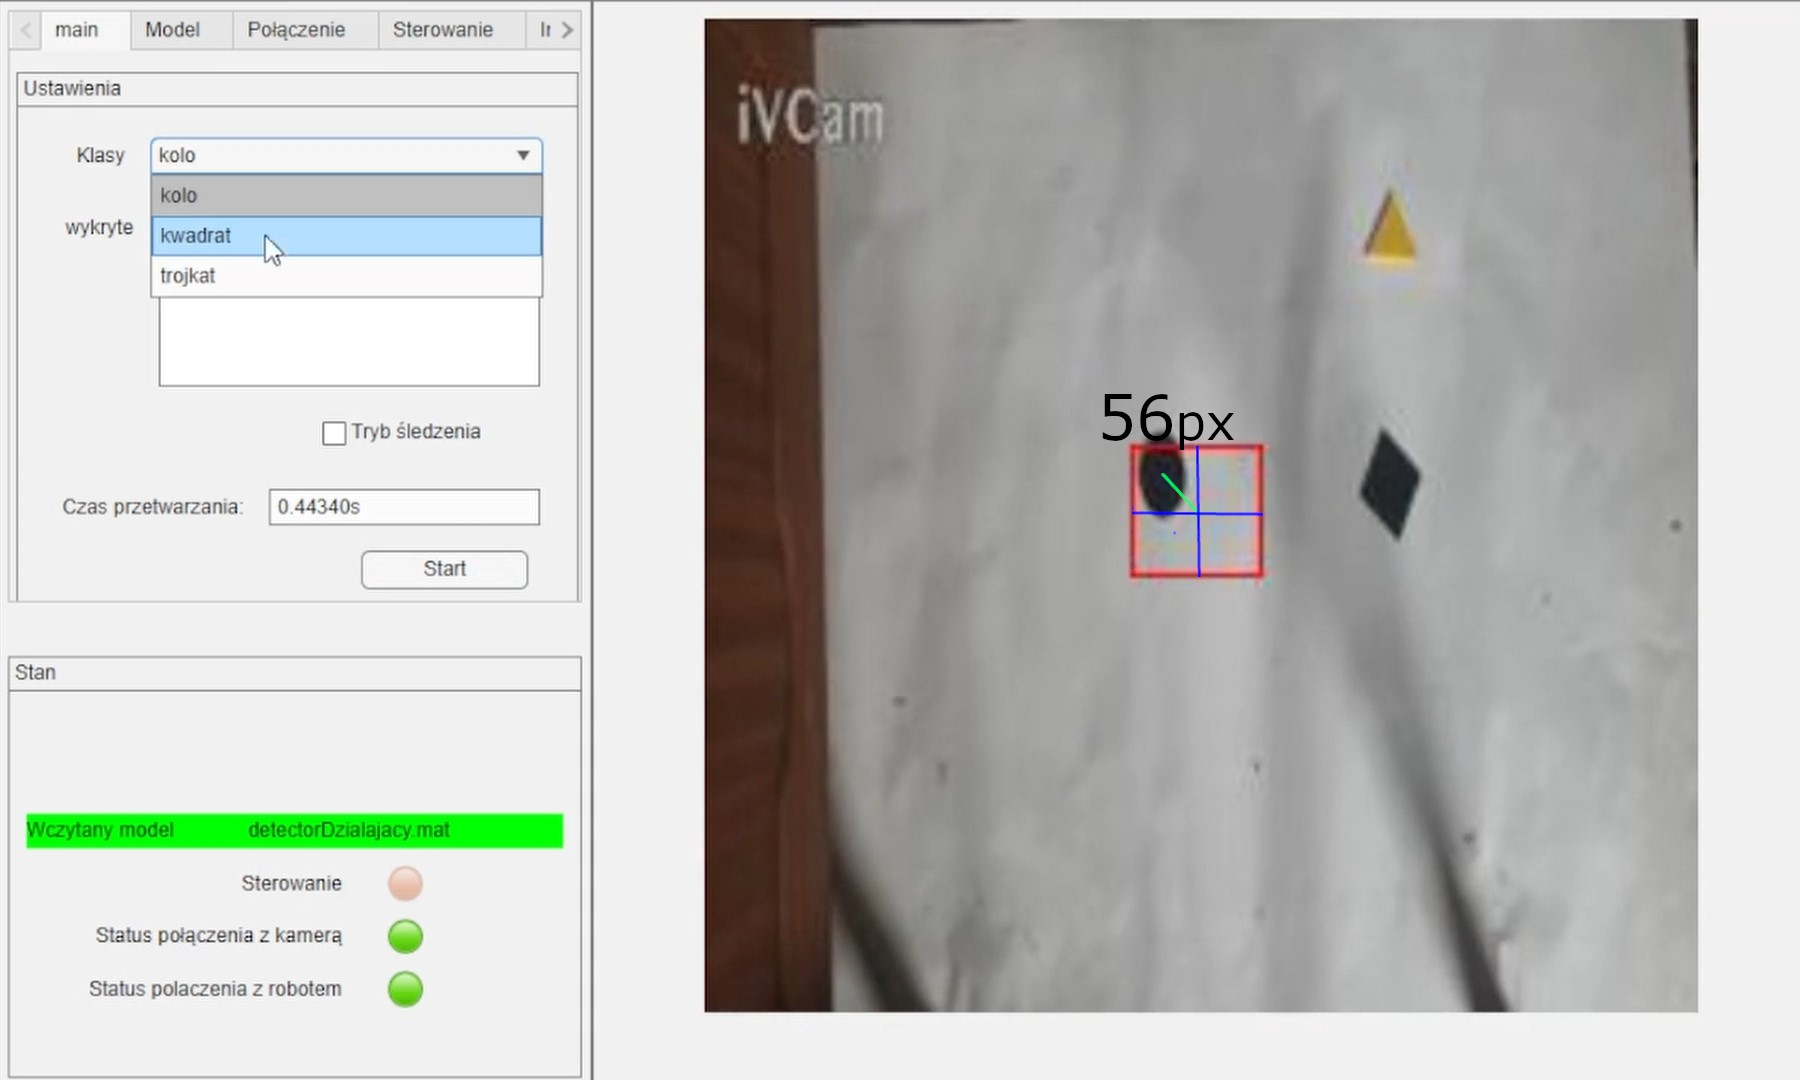
\includegraphics[width=14cm]{pages/testy/img/test1_3.jpg}
	\caption{Test trybu normalnego - znalezienie koła}
\end{figure}
Ostatni przeprowadzony test polegał na znalezieniu koła. Ponownie, jak w poprzednich przypadkach, pojawił się względnie spory błąd w wyśledzonym obiekcie. 
Analizując wszystkie te przypadki, można zauważyć, że błąd ten rośnie wraz ze zwiększeniem się odległości pomiędzy pozycją startową a końcową.
Prawdopodobnie w głównej mierze wynika to z nie dokładnie dobranego współczynników p w regulatorze wyznaczającym przesunięcie.
Warto zauważyć, że w tym trybie algorytm potrzebuje średnio około 400-500ms na analizę obrazu.
\subsection{Testy trybu śledzenia}
W związku z błędami widocznymi w poprzednim teście, opracowano drugą wersję algorytmu, który uruchomiony był w pętli 
i ciągle kompensował błędy pozycjonowania. Nazwany został śledzącym, przez to, że potrafi aktywnie śledzić dynamicznie poruszający się po scenie obiekt.
Aby uruchomić ten tryb, należy wykonać te same kroki co w poprzedniej wersji, jednak przed uruchomieniem należy zaznaczyć opcje tryb śledzenia.
\begin{figure}[H]
	\centering
	\begin{subfigure}{}
		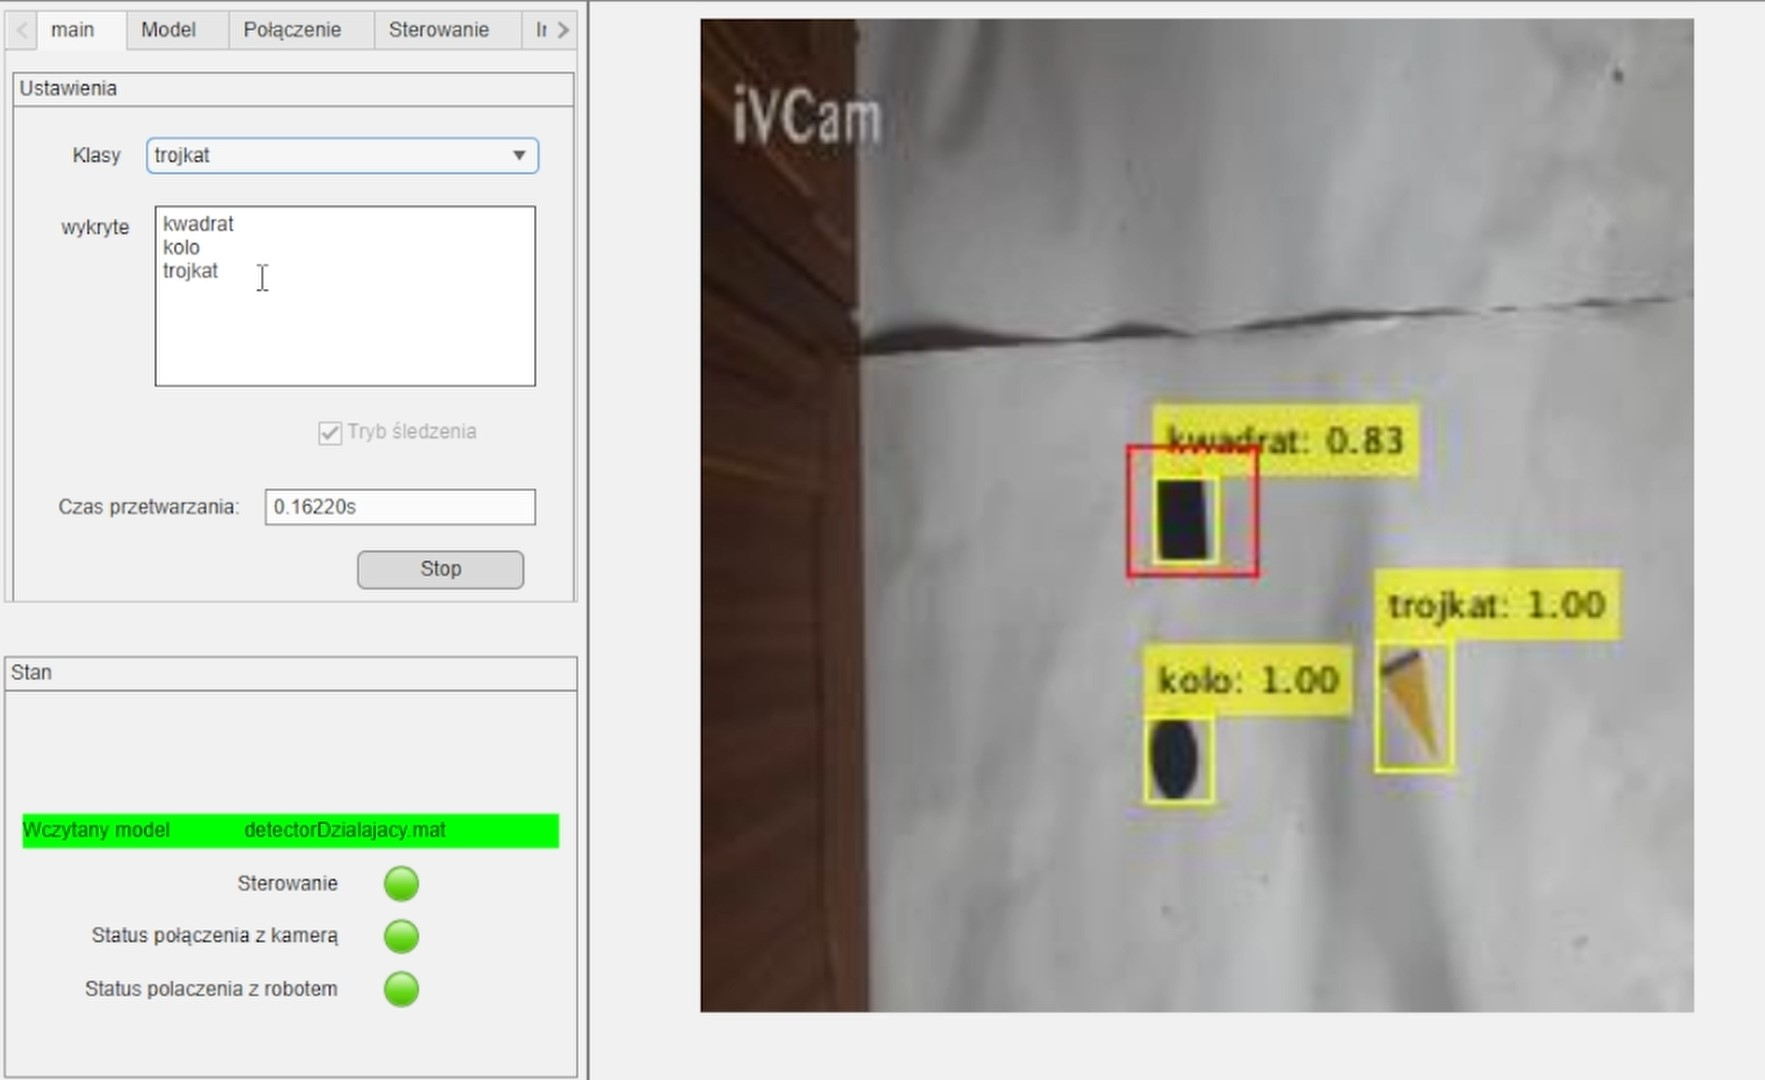
\includegraphics[width=0.5\linewidth]{pages/testy/img/test2_1_2.jpg}
	\end{subfigure}
	\begin{subfigure}{}
		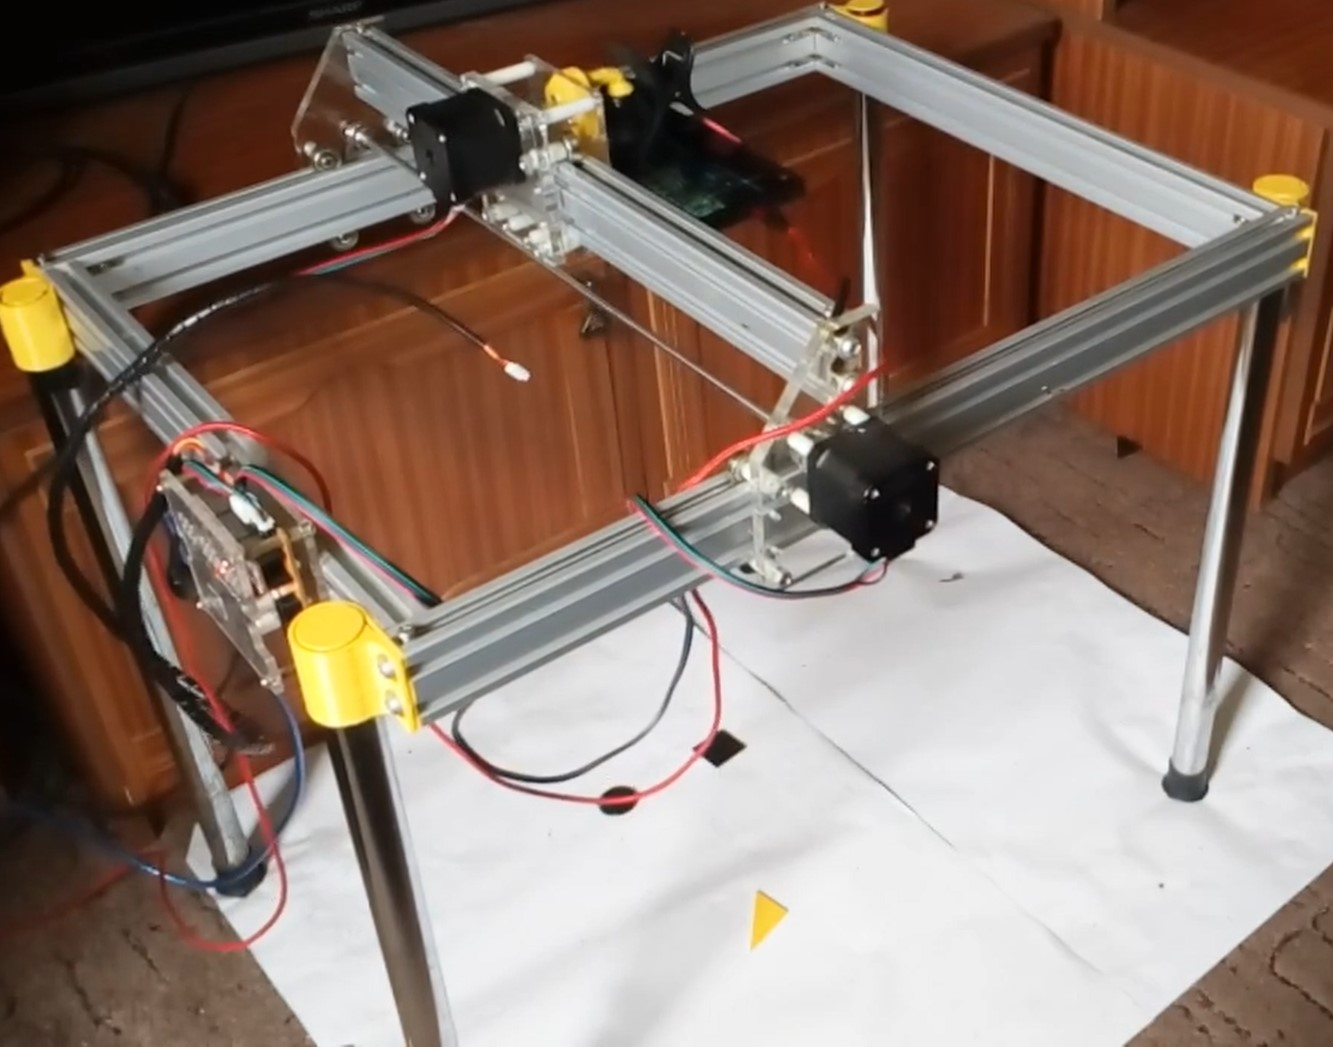
\includegraphics[width=0.4\linewidth]{pages/testy/img/test2_1_1.jpg}
	\end{subfigure}
	\caption{Tryb śledzący, widok z programu i boku robota}
\end{figure}
Jak widać w tym przypadku, sieć neuronowa analizuje każdą klatkę obrazu (widoczne są wykryte obiekty). 
Dzięki ciągłej korekcji błędów, docelowy kształt znajduje się praktycznie idealnie na środku, a po ręcznym przesunięciu
 pozycja jest automatycznie korygowana. Warto zwrócić uwagę na czas przetwarzania, który wynosi około 110ms, 
 co jest znacznie lepszym wynikiem w porównaniu do poprzedniego trybu. 
 \begin{figure}[H]
	\centering
	\begin{subfigure}{}
		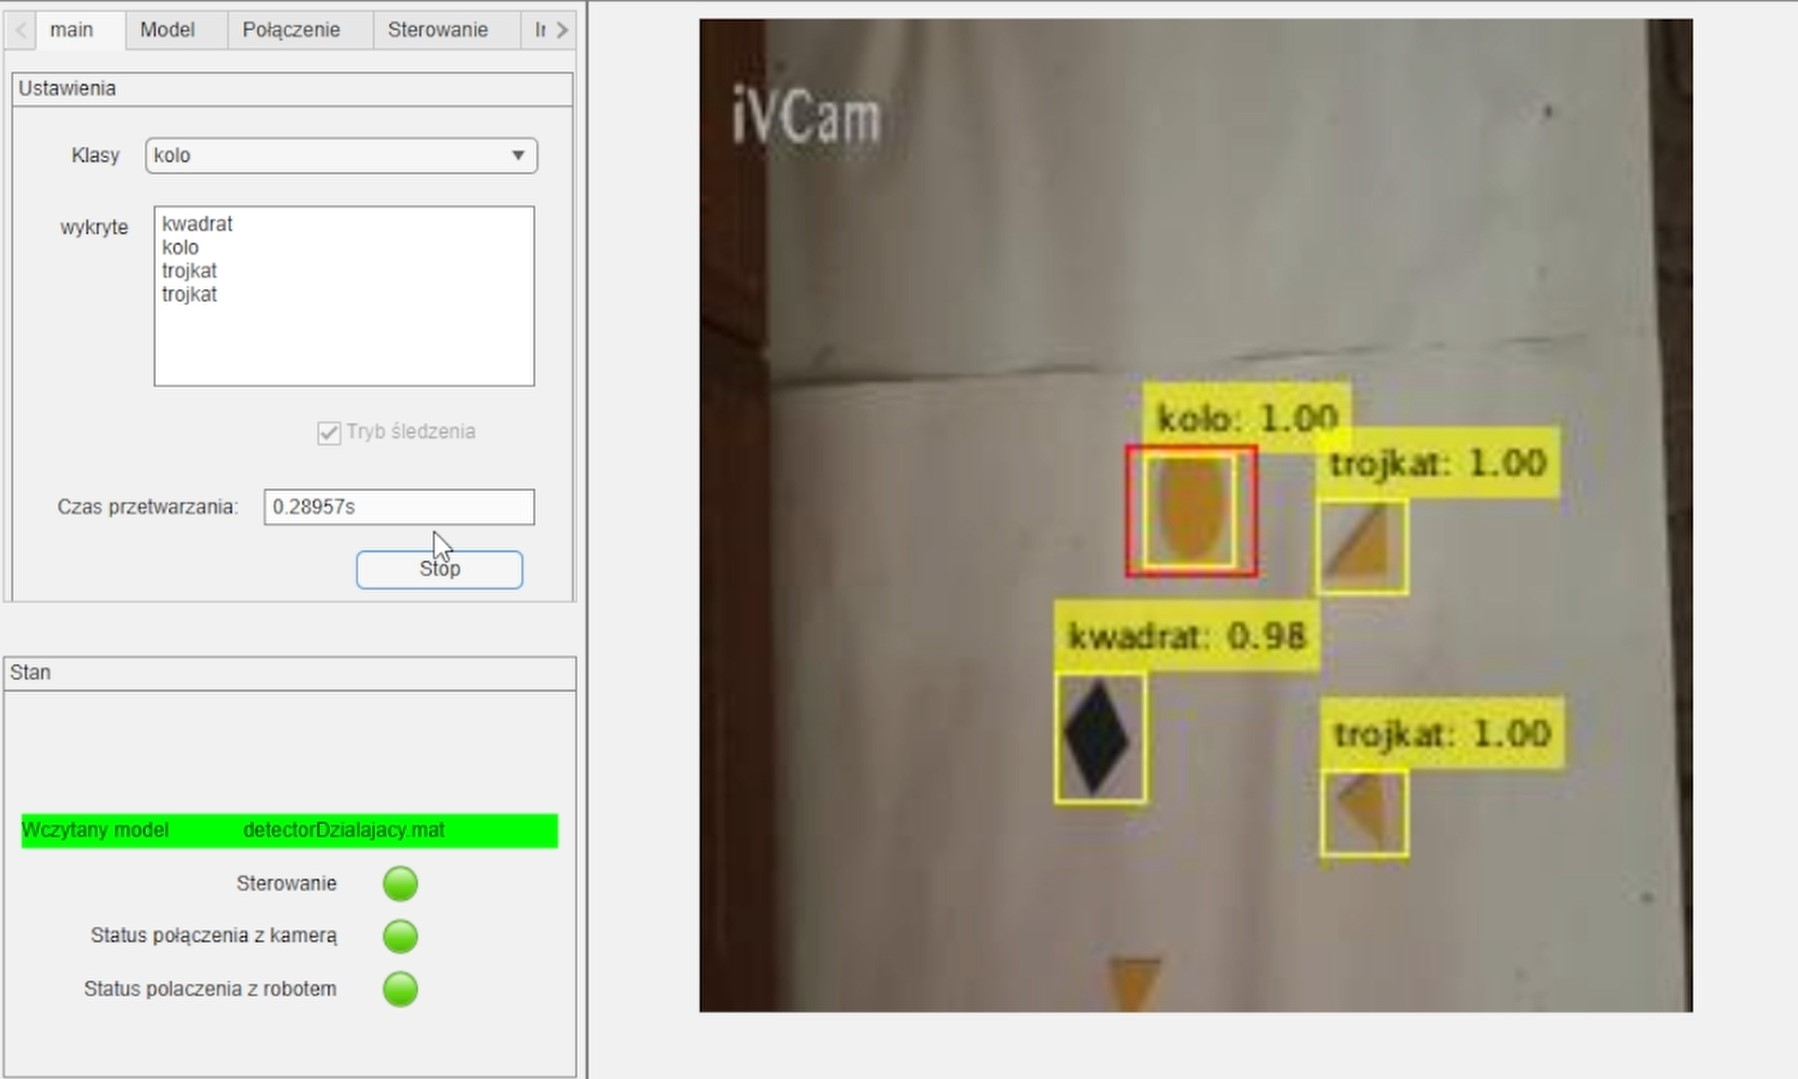
\includegraphics[width=0.5\linewidth]{pages/testy/img/test2_2_2.jpg}
	\end{subfigure}
	\begin{subfigure}{}
		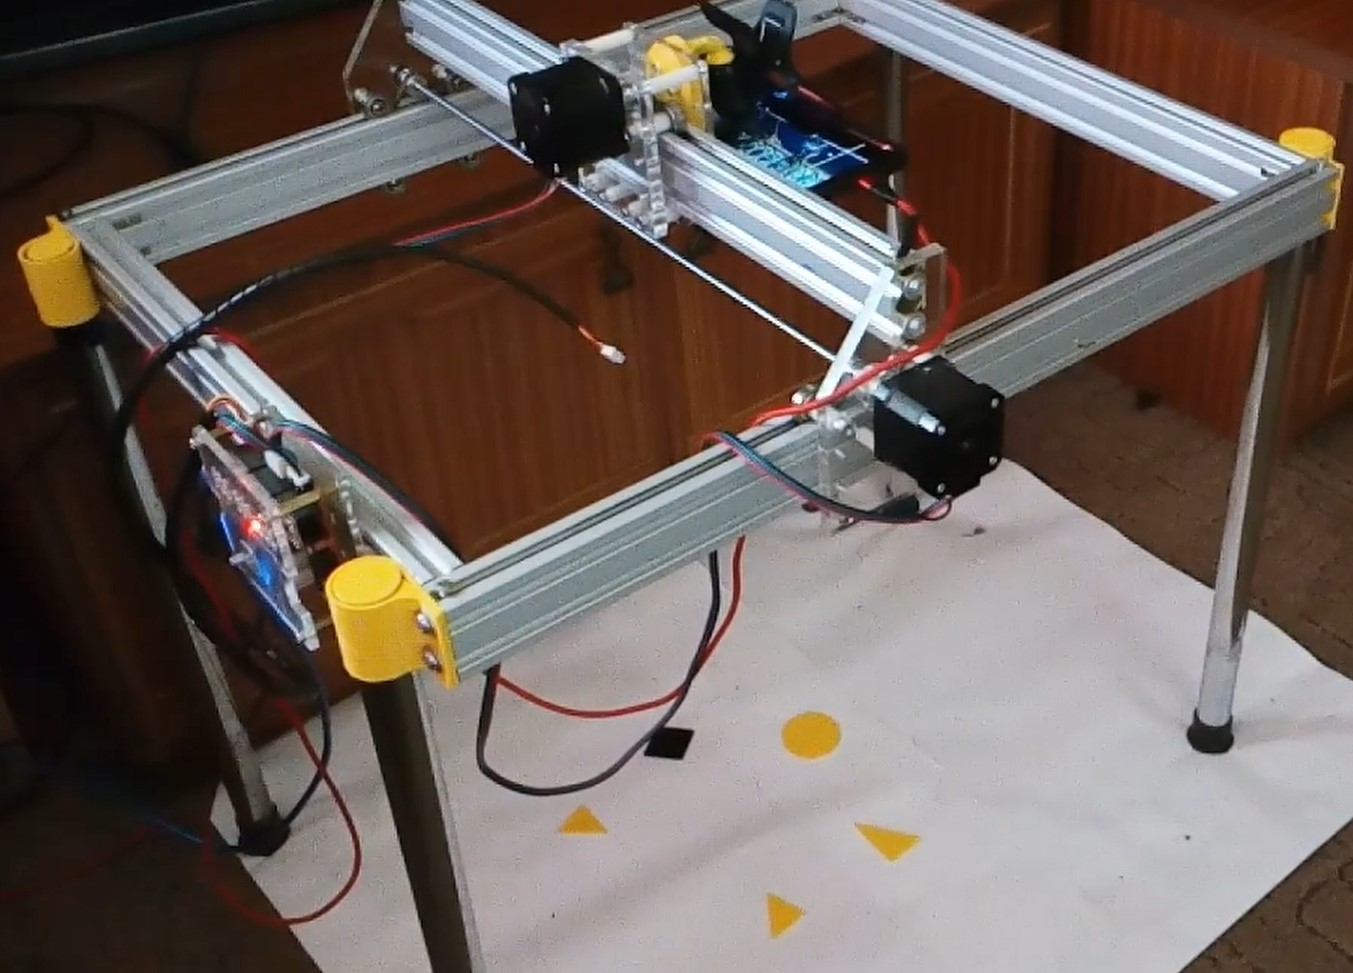
\includegraphics[width=0.4\linewidth]{pages/testy/img/test2_2_1.jpg}
	\end{subfigure}
	\caption{Śledzenie koła}
\end{figure}
Podobnie jak poprzednio, śledzenie koła działa równie dobrze, a osiągane błędy są bardzo małe. 
W porównaniu do poprzedniego trybu, w tym widoczne są duże różnice w sposobie sterowania. W pierwszej wersji algorytmu, cały ruch wykonywany był za jednym razem, a w trybie śledzenia pozycja zmieniana jest w małych krokach.

\section{Podsumowanie}
\textbf{Budowa robota} \newline
Analizując pracę i konstrukcję zbudowanego robota, można zauważyć, że ogólnie konstrukcja spełniła podstawowe założenia 
pracy inżynierskiej, jednak można poprawić konstrukcje w wielu miejscach. 
Podczas finalnej pracy i testowania roboczej wersji algorytmu, gdy ten posiadał sporo błędów, przydatne okazałyby się czujniki krańcowe, które nie pozwoliłyby 
na próbę wyjazdu karetki robota poza poprawny obszar pracy. Takie wjazdy bardzo zmniejszają żywotność silników, ich sterowników (duży płynący przez uzwojenie prąd) oraz 
mechanicznych elementów, takich jak paski czy łożyska. 

Kolejne konstrukcyjne ulepszenie powinno skupić się na zwiększeniu sztywności 
nóg utrzymujących ramę. Uzyskana sztywność była wystarczająca, jednak podczas szybkich i gwałtownych ruchów robota było widoczne chybotanie się 
całej konstrukcji. 


Największym problemem okazało się sterowanie w otwartej pętli, które powodowało spore błędy w sterowaniu 'jednorazowym'. 
Błędy te były spowodowane w znacznej części przez niedokładnie dobrany współczynnik skali oraz przez brak 'świadomości' robota
o własnej pozycji i korygowanie jej względem oczekiwanej. 


Aby poprawić ten błąd należałoby dodać do silników enkodery oraz system pozycjonowania (np. dojazd do rogu robota i określenie tej pozycji jako 0,0),
dzięki czemu byłoby możliwe uruchomienie sterowania ze sprzężeniem zwrotnym.
Dodatkowo dzięki dodaniu systemu pozycjonowania, algorytm śledzący mógłby dokładniej wyznaczać docelowe koordynaty oraz 
monitorować je w trakcie pracy. 

Powyższe błędy udało się zminimalizować trybem "śledzenia", które aktywnie w trakcie pracy kompensowało 
błędy wynikające w wyżej wymienionych niedokładności.

\textbf{Sieć neuronowa i algorytm sterowania} \newline
Podobnie jak w przypadku fizycznej części robota, udało się osiągnąć założony efekt, jednak w trakcie rozwoju pojawiło się sporo 
miejsca na usprawnienia. Uważam, że wytrenowana sieć neuronowa bardzo dobrze radzi sobie z wykrywaniem danych obiektów i to niezależnie od ich 
orientacji, położenia, koloru czy konfiguracji (np. różne typy trójkątów). Analizując model sieci neuronowej, można dojść do wniosku,
że jest ona zbyt dużą i powolna jak na tak proste zadanie i rozpoznawanie figur geometrycznych. 


Kolejny projekt powinien bazować na zdecydowanie mniejszej 
sieci neuronowej (np. opisana w rozdziale \ref{section:architekturaAlgorytmu} architektura sieci tiny-yoloV4), co pozwoliłoby zwiększenie szybkości przetwarzania, zwłaszcza na słabszym komputerze, np. Rassbery Pi.


Kolejnym usprawnieniem, jakie można wprowadzić to dodanie danych z obiektami będącymi na zróżnicowanym tle, co pozwoliłoby na działanie 
w zdecydowanie bardziej zróżnicowanych warunkach.


Posiadając już doświadczenie z tworzeniem aplikacji okienkowych w Matlabie, uważam że komercyjne rozwiązanie powinno być napisane 
przy pomocy zdecydowanie wydajniejszego językam takiego jak C++ lub podobnego. Ze względu na bardzo szerokie zastosowanie Matlaba, wygenerowana aplikacja 
zajmowała bardzo dużo miejsca na dysku, a zapisywany model mógłby być ograniczony jedynie do wag sieci, co zmniejszyło by jego uniwersalność w modyfikacji, 
ale poprawiło zużycie dysku. Dodatkowo dzięki zastosowaniu  technologi CUDA, można byłoby lepiej wykorzystać dostępne sprzętowe zasoby.


\clearpage
\addcontentsline{toc}{section}{Literatura}
\begin{thebibliography}{4}
	\bibitem{sztucznyNeuron} https://batmaja.com/sztuczny-neuron/ Dostęp: 07.01.2023 
	\bibitem{schematAISite} https://www.v7labs.com/blog/machine-learning-guide Dostęp: 07.01.2023 
	\bibitem{matlabDetekcjaPrzyklad} https://www.mathworks.com/help/vision/ug/object-detection-using-yolov4-deep-learning.html Dostęp: 26.01.2023 
	\bibitem{rcnnAndFRCNNTowards} https://towardsdatascience.com/r-cnn-fast-r-cnn-faster-r-cnn-yolo-object-detection-algorithms-36d53571365e Dostęp: 06.06.2023 
	\bibitem{yoloV3ArtAutora} Joseph Redmon, Ali Farhadi "YOLOv3: An Incremental Improvement", University of Washington 2018 
	\bibitem{yoloAndMobileRobot}Douglas Henke Dos Reis,  Mobile Robot Navigation Using an Object Recognition Software with RGBD Images and the YOLO Algorithm DOI: 10.1080/08839514.2019.1684778
	\bibitem{grblGithub} Projekt grbl, https://github.com/gnea/grbl/ Dostęp 08.06.2023r 
	\bibitem{matlabOYolov4} https://www.mathworks.com/help/vision/ug/getting-started-with-yolo-v4.html Dostęp 04.06.2023 
\end{thebibliography}

\clearpage
\end{document} 